%% Template Laporan Tugas Besar Sistem Pemberi Rekomendasi (CAK4TBB3)
%% Fakultas Informatika, Universitas Telkom
%% Berbasis Template Proposal FIF Telkom University

\documentclass[a4paper,12pt,oneside]{book}
\usepackage[utf8]{inputenc}
\usepackage{lmodern}
\usepackage{sectsty}
\usepackage{graphicx}
\usepackage{epstopdf}
\usepackage{algorithm}
\usepackage{algpseudocode}
\usepackage{array}
\usepackage[table]{xcolor}
\usepackage{anysize}
\usepackage{amsmath}
\usepackage{amssymb}
\usepackage[bahasa]{babel}
\usepackage{indentfirst} % Spasi untuk paragraf pertama
\usepackage{geometry}
\usepackage{multirow}
\usepackage{hhline}
\usepackage{booktabs}
\usepackage{tabularx}
\usepackage{longtable}
\marginsize{4cm}{3cm}{3cm}{3cm} % {left}{right}{top}{bottom}
\usepackage[compact]{titlesec} 
\usepackage{etoolbox}
\usepackage{natbib} % for Harvard/numeric style
\usepackage[bookmarks,hypertexnames=false,debug]{hyperref}
\usepackage{bookmark}

% Path direktori gambar
\graphicspath{{figures/}{../figures/}{./}}

\makeatletter
\patchcmd{\ttlh@hang}{\parindent\z@}{\parindent\z@\leavevmode}{}{}
\patchcmd{\ttlh@hang}{\noindent}{}{}{}
\makeatother

\chapterfont{\centering}
\newcommand{\bigsize}{\fontsize{16pt}{14pt}\selectfont}
\chapterfont{\centering\bigsize\bfseries}
\sectionfont{\large\bfseries}
\usepackage{tikz}
\usetikzlibrary{shapes.geometric, arrows}

\renewcommand{\thechapter}{\Roman{chapter}}
\renewcommand\thesection{\arabic{chapter}.\arabic{section}}
\renewcommand\thesubsection{\thesection.\arabic{subsection}}
\renewcommand{\theequation}{\arabic{chapter}.\arabic{equation}}
\renewcommand{\thefigure}{\arabic{chapter}.\arabic{figure}}
\renewcommand{\thetable}{\arabic{chapter}.\arabic{table}}

\renewcommand\bibname{Daftar Pustaka}
\addto{\captionsbahasa}{\renewcommand{\bibname}{Daftar Pustaka}}
\usepackage{fancyhdr}
\pagestyle{fancy}
\lhead{}
\chead{}
\rhead{}
\lfoot{}
\cfoot{\thepage}
\rfoot{}
\renewcommand{\headrulewidth}{0pt}

\makeatletter

%%%%%%%%%%%%%%%%%%%%%%%%%%%%%%%%%%%%%%%%%%%%%%%%%%%%%%%%%%%%
% Metadata Tugas Kelompok 3
%%%%%%%%%%%%%%%%%%%%%%%%%%%%%%%%%%%%%%%%%%%%%%%%%%%%%%%%%%%%
\title{EVALUASI SISTEM PEMBERI REKOMENDASI: STUDI KOMPARATIF COLLABORATIVE FILTERING DAN MATRIX FACTORIZATION PADA MOVIELENS 100K}\let\Title\@title

\newcommand{\EngTitle}{Evaluation of Recommender Systems: A Comparative Study of Collaborative Filtering and Matrix Factorization on MovieLens 100K}

\author{Kelompok 3} \let\Author\@author
\newcommand{\Prodi}{Informatika}
\newcommand{\MataKuliah}{Sistem Pemberi Rekomendasi (CAK4TBB3)}
\newcommand{\SubCLO}{Sub-CLO 12-1-1: Evaluasi Sistem Rekomendasi}
\newcommand{\Kelas}{IF-47-01 / RecSys 2627-1}
\newcommand{\Dosen}{Prof. Dr. Z.K. Abdurahman Baizal, S.Si., M.Kom.}
\date{2026} \let\Date\@date

\makeatother
\linespread{1.15}

\begin{document}

%%%%%%%%%%%%%%%%%%%%%%%%%%%%%%%%%%%%%%%%%%%%%%%%%%%%%%%%%%
% Bagian Awal: Cover, Abstrak, Daftar Isi
%%%%%%%%%%%%%%%%%%%%%%%%%%%%%%%%%%%%%%%%%%%%%%%%%%%%%%%%%%
\pagenumbering{roman} 
\begin{titlepage}
\thispagestyle{empty}
\pdfbookmark{Cover}{ }
\begin{center}
% 1. LAPORAN TUGAS BESAR & MATA KULIAH
{\large\bfseries LAPORAN TUGAS BESAR\par}
\vspace{0.15cm}
{\large\bfseries \MataKuliah\par}
\vspace{0.15cm}
{\normalsize\bfseries \SubCLO\par}
{\normalsize\bfseries Kelas: \Kelas\par}

\vspace{0.6cm}
% 2. JUDUL
{\fontsize{13pt}{16pt}\selectfont\bfseries \Title\par}

\vspace{0.6cm}
% 3. LOGO

\includegraphics[height=3.0cm]{Tel-U-Logo}

\vspace{0.6cm}
% 4. DOSEN PENGAMPU
{\normalsize\bfseries Dosen Pengampu:\par}
\vspace{0.1cm}
{\normalsize \Dosen\par}

\vspace{0.5cm}
% 5. IDENTITAS KELOMPOK
{\normalsize\bfseries Disusun Oleh: Kelompok 3\par}
\vspace{0.2cm}
{\footnotesize
\begin{tabular}{c l c}
\toprule
\textbf{No} & \textbf{Nama Mahasiswa} & \textbf{NIM} \\
\midrule
1 & Daffa Irsandy Putra & 103012300338 \\
2 & Alvito Buana & 103012300232 \\
3 & Zweta Lathifah Kus Aliyyah & 103012300107 \\
4 & Muhammad Ragil & 103012300015 \\
5 & Laili Faisa Dwi Cahyarini & 103012300431 \\
\bottomrule
\end{tabular}
\par}

\vfill

% 6. IDENTITAS KAMPUS
{\normalsize\bfseries Program Studi Sarjana \Prodi\par}
{\normalsize\bfseries Fakultas Informatika\par}
{\normalsize\bfseries Universitas Telkom\par}
{\normalsize\bfseries Bandung\par}
{\normalsize\bfseries \Date\par}
\end{center}

\end{titlepage}

\phantomsection
\addcontentsline{toc}{chapter}{Abstrak}
\chapter*{Abstrak}

Ledakan informasi dalam platform hiburan digital menuntut sistem pemberi rekomendasi yang mampu memprediksi preferensi pengguna secara akurat di tengah tingginya tingkat kelangkaan data (\textit{data sparsity}). Penelitian ini menyajikan evaluasi komparatif komprehensif terhadap algoritma perekomendasi berbasis \textit{collaborative filtering} pada dataset MovieLens 100K (943 pengguna, 1.682 film, 100.000 rating, sparsitas 93,70\%) dengan skema protokol baku 5-\textit{fold cross-validation}. Seluruh algoritma dan metrik diimplementasikan secara modular dari awal (\textit{from scratch}) tanpa pustaka rekomendasi pihak ketiga, mencakup empat model \textit{baseline} (tebak acak, rata-rata global, rata-rata pengguna, dan rata-rata film), dua metode \textit{memory-based} (User-Based Collaborative Filtering dengan korelasi Pearson dan Item-Based Collaborative Filtering dengan \textit{adjusted cosine}), serta metode \textit{model-based} Matrix Factorization berbasis \textit{Stochastic Gradient Descent} (SGD) dengan regularisasi $L_2$. Evaluasi diukur melalui metrik kesalahan rating (MAE, MSE, RMSE, NMSE) dan kemampuan perankingan (NDCG@10). Hasil eksperimen menunjukkan bahwa \textit{baseline} rata-rata film merupakan acuan terkuat (MAE 0,8174; RMSE 1,0246; NDCG@10 0,8329). Metode User-Based CF menghasilkan MAE terendah (0,7342, perbaikan 10,18\% dibanding \textit{baseline}). Sementara itu, Matrix Factorization unggul secara konsisten dan signifikan pada seluruh lima \textit{fold} untuk metrik RMSE (0,9249, perbaikan 9,73\%, $p = 0,0002$ pada uji t berpasangan) serta kualitas perankingan daftar rekomendasi NDCG@10 (0,8578, perbaikan 2,99\%, $p = 0,0102$). Selain itu, Matrix Factorization menawarkan latensi prediksi tercepat (0,014 detik), menjadikannya kandidat paling optimal untuk deployment sistem rekomendasi skala besar.

\vspace{0.5 cm}
\begin{flushleft}
{\textbf{Kata Kunci:} Sistem Pemberi Rekomendasi, Collaborative Filtering, Matrix Factorization, MovieLens 100K, Evaluasi 5-Fold Cross Validation.}
\end{flushleft}

\clearpage

\phantomsection
\addcontentsline{toc}{chapter}{Daftar Isi}
\tableofcontents
\cleardoublepage

\phantomsection
\addcontentsline{toc}{chapter}{Daftar Gambar}
\listoffigures
\cleardoublepage

\phantomsection
\addcontentsline{toc}{chapter}{Daftar Tabel}
\listoftables
\cleardoublepage

%%%%%%%%%%%%%%%%%%%%%%%%%%%%%%%%%%%%%%%%%%%%%%%%%
% Bab-bab Laporan
%%%%%%%%%%%%%%%%%%%%%%%%%%%%%%%%%%%%%%%%%%%%%%%%%
\pagenumbering{arabic}
\chapter{Pendahuluan}

\section{Latar Belakang}
Perkembangan pesat platform digital dan layanan media \textit{streaming} telah memicu fenomena ledakan informasi (\textit{information overload}), di mana jutaan konten tersedia secara simultan sementara kapasitas atensi kognitif manusia bersifat terbatas \citep{ricci2015recommender}. Dalam konteks platform hiburan film, pengguna kerap menghadapi kesulitan memilih film yang sesuai dengan preferensi personal di antara ribuan judul yang tersedia. Sistem Pemberi Rekomendasi (\textit{Recommender System}) hadir sebagai solusi teknologi krusial yang menyaring volume konten masif dan menghadirkan saran personalisasi yang relevan \citep{jannach2010recommender}.

Pendekatan paling dominan dan berhasil diterapkan dalam industri rekomendasi adalah \textit{Collaborative Filtering} (CF) \citep{su2009survey}. Berbeda dengan \textit{Content-Based Filtering} yang bergantung pada ekstraksi atribut deskriptif item (seperti genre, sutradara, atau sinopsis), \textit{Collaborative Filtering} murni memanfaatkan pola interaksi masa lalu antara pengguna dan item. Paradigma CF terbagi menjadi dua mazhab utama:
\begin{enumerate}
    \item \textbf{Memory-Based Collaborative Filtering}: Menggunakan seluruh matriks interaksi pengguna-item secara langsung untuk menghitung derajat kemiripan. Pendekatan ini terbagi menjadi \textit{User-Based Collaborative Filtering} (UBCF) yang memprediksi preferensi berdasarkan pengguna lain yang memiliki pola rating serupa \citep{resnick1994grouplens}, dan \textit{Item-Based Collaborative Filtering} (IBCF) yang mengestimasi rating berdasarkan kemiripan historis antar-item yang telah dinilai oleh pengguna yang sama \citep{sarwar2001item}.
    \item \textbf{Model-Based CF}: Mengonstruksi representasi matematis laten dari data interaksi. Algoritma \textit{Matrix Factorization} (MF) yang dipopulerkan pada kompetisi Netflix Prize merepresentasikan pengguna dan item ke dalam ruang faktor laten berdimensi rendah ($K \ll \min(|U|, |I|)$), dioptimalkan menggunakan \textit{Stochastic Gradient Descent} (SGD) dengan regularisasi $L_2$ \citep{koren2009matrix}.
\end{enumerate}

Meskipun ketiga metode tersebut sangat populer, implementasi praktisnya menghadapi tantangan serius berupa tingginya tingkat kekosongan matriks (\textit{data sparsity}). Pada dataset tolok ukur MovieLens 100K \citep{harper2015movielens}, tingkat kelangkaan data mencapai 93,70\%, yang berarti hanya sekitar 6,30\% kombinasi pengguna-item yang memiliki rating eksplisit. Kondisi sparsitas ekstrem ini berdampak langsung pada keakuratan perhitungan kemiripan tetangga pada metode \textit{memory-based} serta risiko \textit{overfitting} pada metode \textit{model-based}.

Selain tantangan data, aspek evaluasi sistem rekomendasi sering kali dipersempit hanya pada metrik kesalahan rating absolut seperti \textit{Mean Absolute Error} (MAE) atau \textit{Root Mean Squared Error} (RMSE). Padahal, dalam skenario nyata, pengguna tidak semata-mata membutuhkan prediksi angka rating yang akurat, melainkan daftar rekomendasi teratas (\textit{Top-N Recommendation}) yang benar-benar relevan dan terurut secara tepat \citep{jarvelin2002cumulated}. Oleh karena itu, evaluasi komprehensif yang mengombinasikan metrik kesalahan prediksi (MAE, MSE, RMSE, NMSE), metrik perankingan (\textit{Normalized Discounted Cumulative Gain} pada $k=10$ atau NDCG@10), serta analisis waktu komputasi merupakan kebutuhan mutlak \citep{baizal2024recsys}.

Penelitian ini dilakukan dalam rangka memenuhi Capaian Pembelajaran Sub-CLO 12-1-1 pada mata kuliah Sistem Pemberi Rekomendasi di Fakultas Informatika Universitas Telkom. Seluruh algoritma, model \textit{baseline}, dan fungsi metrik diimplementasikan secara mandiri dari awal (\textit{from scratch}) tanpa memanfaatkan pustaka sistem rekomendasi siap pakai seperti \textit{Surprise} atau \textit{LightFM}. Pengujian dilakukan menggunakan protokol baku 5-\textit{fold cross-validation} resmi pada MovieLens 100K guna menjamin validitas ilmiah, reproduktibilitas hasil, dan ketelitian analisis komparatif.

\section{Perumusan Masalah}
Berdasarkan latar belakang yang telah dipaparkan, perumusan masalah dalam penelitian ini dijabarkan ke dalam empat poin pertanyaan penelitian:
\begin{enumerate}
    \item Bagaimana akurasi prediksi rating dari metode \textit{User-Based Collaborative Filtering} (UBCF), \textit{Item-Based Collaborative Filtering} (IBCF), dan \textit{Matrix Factorization} (MF) dibandingkan dengan empat model \textit{baseline} (tebak acak, rata-rata global, rata-rata pengguna, dan rata-rata film) pada dataset MovieLens 100K?
    \item Bagaimana pengaruh ukuran ketetanggaan ($k$) pada UBCF dan IBCF terhadap kinerja kesalahan estimasi rating?
    \item Bagaimana efektivitas masing-masing pendekatan rekomendasi dalam menghasilkan urutan rekomendasi Top-10 yang relevan berdasarkan metrik perankingan \textit{Normalized Discounted Cumulative Gain} (NDCG@10)?
    \item Bagaimana karakteristik \textit{trade-off} antara akurasi prediksi (MAE, RMSE), kualitas perankingan (NDCG@10), dan efisiensi waktu komputasi (waktu pelatihan dan waktu inferensi) antar algoritma yang diuji?
\end{enumerate}

\section{Tujuan Penelitian}
Tujuan yang hendak dicapai dalam pelaksanaan tugas besar penelitian ini adalah:
\begin{enumerate}
    \item Mengimplementasikan dan mengevaluasi kinerja empat model \textit{baseline}, UBCF, IBCF, dan Matrix Factorization pada dataset MovieLens 100K menggunakan protokol baku 5-\textit{fold cross-validation}.
    \item Melakukan analisis sensitivitas parameter ukuran ketetanggaan ($k$) pada UBCF dan IBCF guna mengidentifikasi nilai parameter optimal.
    \item Mengukur dan membandingkan kualitas perankingan daftar rekomendasi Top-10 antar metode menggunakan metrik NDCG@10 dengan ambang batas kepuasan biner $r \ge 4$.
    \item Melakukan analisis komparatif menyeluruh mencakup akurasi prediksi, perankingan, uji signifikansi statistik berpasangan (\textit{paired t-test}), sebaran residual error, dampak sparsitas data, dan kompleksitas waktu komputasi untuk memberikan rekomendasi pemilihan arsitektur sistem perekomendasi film.
\end{enumerate}

\section{Ruang Lingkup dan Batasan}
Ruang lingkup dan batasan penelitian ini ditetapkan sebagai berikut:
\begin{enumerate}
    \item \textbf{Dataset}: Menggunakan dataset publik resmi MovieLens 100K yang dirilis oleh GroupLens Research, terdiri atas 100.000 rating dari 943 pengguna terhadap 1.682 film dalam rentang skala rating diskrit bilangan bulat 1 sampai 5.
    \item \textbf{Protokol Evaluasi}: Menggunakan partisi resmi 5-\textit{fold cross-validation} bawaan MovieLens (\texttt{u1.base}/\allowbreak\texttt{u1.test} sampai \texttt{u5.base}/\allowbreak\texttt{u5.test}) dengan rasio 80:20 pada tiap \textit{fold}.
    \item \textbf{Batasan Pustaka}: Seluruh algoritma perekomendasi, perhitungan kesamaan, optimasi SGD, dan metrik evaluasi diimplementasikan murni dari awal menggunakan bahasa pemrograman Python 3.12 dengan bantuan pustaka komputasi numerik NumPy, Pandas, dan SciPy, tanpa menggunakan kerangka kerja rekomendasi siap pakai (\textit{black-box}).
    \item \textbf{Metrik Evaluasi}: Evaluasi kuantitatif mencakup metrik kesalahan prediksi rating: MAE (\textit{Mean Absolute Error}), MSE (\textit{Mean Squared Error}), RMSE (\textit{Root Mean Squared Error}), NMSE (\textit{Normalized Mean Squared Error}), serta metrik kualitas perankingan NDCG@10 (\textit{Normalized Discounted Cumulative Gain} pada $k=10$).
    \item \textbf{Lingkungan Eksekusi}: Pengujian dilakukan pada lingkungan perangkat keras prosesor tunggal (CPU) standar untuk memastikan keterbandingan waktu komputasi yang adil dan objektif.
\end{enumerate}

\section{Sistematika Penulisan}
Laporan tugas besar ini disusun secara sistematis dengan struktur sebagai berikut:
\begin{itemize}
    \item \textbf{Bab I Pendahuluan}: Memaparkan latar belakang, perumusan masalah, tujuan, batasan ruang lingkup penelitian, serta sistematika penulisan.
    \item \textbf{Bab II Kajian Pustaka}: Menguraikan landasan teori mengenai sistem pemberi rekomendasi, karakteristik matriks interaksi, formulasi matematis UBCF, IBCF, Matrix Factorization, metrik evaluasi rating dan ranking, serta pengujian statistik.
    \item \textbf{Bab III Metodologi dan Desain Sistem}: Menjelaskan diagram alur penelitian, spesifikasi dataset, skenario model \textit{baseline}, rancangan pengujian algoritma rekomendasi, dan strategi verifikasi kode (\textit{sanity check}).
    \item \textbf{Bab IV Hasil dan Pembahasan}: Menyajikan hasil eksplorasi data (EDA), perbandingan kinerja 5-\textit{fold cross-validation}, analisis sensitivitas parameter, kurva belajar SGD, uji signifikansi statistik berpasangan, analisis sebaran residual error, evaluasi waktu komputasi, serta studi kasus Top-10 rekomendasi.
    \item \textbf{Bab V Kesimpulan dan Saran}: Menyimpulkan temuan utama penelitian yang menjawab rumusan masalah dan memberikan saran konstruktif untuk pengembangan sistem di masa mendatang.
\end{itemize}
        % Bab I
\chapter{Kajian Pustaka}

\section{Taksonomi Sistem Rekomendasi dan Karakteristik Data Matriks Interaksi}
Sistem pemberi rekomendasi (\textit{recommender system}) memodelkan interaksi antara himpunan pengguna $U = \{u_1, u_2, \dots, u_{|U|}\}$ dan himpunan item $I = \{i_1, i_2, \dots, i_{|I|}\}$. Interaksi tersebut direpresentasikan ke dalam matriks rating eksplisit $R \in \mathbb{R}^{|U| \times |I|}$, di mana elemen $r_{u,i}$ menyatakan tingkat preferensi yang diberikan oleh pengguna $u$ terhadap item $i$. Pada umumnya, skala rating bernilai diskrit dalam domain tertentu, seperti $\{1, 2, 3, 4, 5\}$ pada dataset MovieLens \citep{harper2015movielens}.

Karakteristik fundamental dari matriks interaksi $R$ adalah tingginya tingkat kekosongan atau sparsitas (\textit{sparsity}) \citep{ricci2015recommender}. Himpunan pasangan pengguna-item yang teramati didefinisikan sebagai $\mathcal{K} = \{(u, i) \mid r_{u,i} \neq \emptyset\}$. Derajat sparsitas matriks dirumuskan sebagai:
\begin{equation}
\label{eq:sparsity}
\text{Sparsitas} = 1 - \frac{|\mathcal{K}|}{|U| \times |I|}
\end{equation}
Pada kondisi di mana sparsitas melampaui 90\%, sistem menghadapi fenomena \textit{cold-start problem} (kesulitan menghasilkan rekomendasi akurat bagi entitas pengguna atau item baru dengan riwayat interaksi minimal) dan distribusi \textit{long-tail} (hanya sebagian kecil item populer yang mendominasi interaksi, sedangkan mayoritas item jarang dievaluasi) \citep{jannach2010recommender}.

\section{User-Based Collaborative Filtering (UBCF)}
\textit{User-Based Collaborative Filtering} (UBCF) didasarkan pada premis bahwa pengguna yang memiliki preferensi serupa di masa lampau cenderung memiliki ketertarikan yang serupa terhadap item di masa depan \citep{resnick1994grouplens}. 

Derajat kesamaan preferensi antara dua pengguna $u$ dan $v$ dihitung menggunakan koefisien korelasi Pearson (\textit{Pearson Correlation Coefficient} / PCC) pada himpunan item yang dinilai bersama $I_{uv} = I_u \cap I_v$:
\begin{equation}
\label{eq:pcc}
\text{sim}(u, v) = \frac{\sum_{i \in I_{uv}} (r_{u,i} - \bar{r}_u)(r_{v,i} - \bar{r}_v)}{\sqrt{\sum_{i \in I_{uv}} (r_{u,i} - \bar{r}_u)^2} \sqrt{\sum_{i \in I_{uv}} (r_{v,i} - \bar{r}_v)^2}}
\end{equation}
di mana $\bar{r}_u$ dan $\bar{r}_v$ masing-masing menyatakan nilai rata-rata rating historis pengguna $u$ dan $v$.

Untuk mencegah bias yang ditimbulkan oleh pasangan pengguna yang hanya mengevaluasi sedikit item bersama ($|I_{uv}|$ kecil), diterapkan teknik pembobotan signifikansi (\textit{significance weighting}) dengan ambang batas $\gamma$:
\begin{equation}
\label{eq:sig_weight_u}
w_{uv} = \text{sim}(u, v) \cdot \frac{\min(|I_{uv}|, \gamma)}{\gamma}
\end{equation}
Setelah menghitung kesamaan, dipilih $k$ pengguna paling mirip yang telah memberikan rating pada item $i$, dinotasikan sebagai himpunan ketetanggaan $N_i(u)$. Nilai estimasi rating $\hat{r}_{u,i}$ dihitung melalui rerata terbobot berbasis deviasi (\textit{deviation-from-mean}):
\begin{equation}
\label{eq:ubcf_pred}
\hat{r}_{u,i} = \bar{r}_u + \frac{\sum_{v \in N_i(u)} w_{uv} (r_{v,i} - \bar{r}_v)}{\sum_{v \in N_i(u)} |w_{uv}|}
\end{equation}
Formulasi deviasi pada Persamaan (\ref{eq:ubcf_pred}) menjamin kompensasi terhadap bias kecenderungan pengguna yang terbiasa memberikan rentang rating tinggi (\textit{optimistic rater}) maupun rendah (\textit{critical rater}).

\section{Item-Based Collaborative Filtering (IBCF)}
\textit{Item-Based Collaborative Filtering} (IBCF) mengatasi kendala komputasi UBCF pada sistem berskala besar di mana jumlah pengguna jauh melampaui jumlah item ($|U| \gg |I|$) \citep{sarwar2001item}. IBCF memprediksi rating pengguna terhadap suatu item berdasarkan rating yang telah diberikan pengguna tersebut pada item-item lain yang serupa.

Penggunaan kesamaan kosinus biasa (\textit{Cosine Similarity}) pada data rating cenderung menghasilkan bias karena mengabaikan disparitas skala penilaian antar-pengguna. Oleh karena itu, digunakan metrik \textit{Adjusted Cosine Similarity} yang mengurangkan rating dengan nilai rata-rata pengguna $\bar{r}_u$ pada himpunan pengguna bersama $U_{ij} = U_i \cap U_j$:
\begin{equation}
\label{eq:adj_cos}
\text{sim}(i, j) = \frac{\sum_{u \in U_{ij}} (r_{u,i} - \bar{r}_u)(r_{u,j} - \bar{r}_u)}{\sqrt{\sum_{u \in U_{ij}} (r_{u,i} - \bar{r}_u)^2} \sqrt{\sum_{u \in U_{ij}} (r_{u,j} - \bar{r}_u)^2}}
\end{equation}
Serupa dengan UBCF, bobot signifikansi dengan parameter penalti $\gamma$ diterapkan untuk item dengan sedikit evaluator bersama:
\begin{equation}
\label{eq:sig_weight_i}
w_{ij} = \text{sim}(i, j) \cdot \frac{\min(|U_{ij}|, \gamma)}{\gamma}
\end{equation}
Estimasi rating $\hat{r}_{u,i}$ dihitung menggunakan kombinasi terbobot dari $k$ item terdekat yang telah dinilai oleh pengguna $u$, dinotasikan sebagai $N_u(i)$:
\begin{equation}
\label{eq:ibcf_pred}
\hat{r}_{u,i} = \frac{\sum_{j \in N_u(i)} w_{ij} \, r_{u,j}}{\sum_{j \in N_u(i)} |w_{ij}|}
\end{equation}

\section{Matrix Factorization berbasis Stochastic Gradient Descent (SGD)}
\textit{Matrix Factorization} (MF) merupakan pendekatan \textit{model-based} yang memetakan pengguna dan item ke dalam ruang faktor laten berdimensi rendah $K$ ($K \ll \min(|U|, |I|)$), sehingga interaksi pengguna-item dimodelkan sebagai hasil perkalian titik (\textit{inner product}) dalam ruang laten tersebut \citep{koren2009matrix}.

Model faktorisasi standar dilengkapi komponen bias untuk menangkap kecenderungan global, bias pengguna, dan bias item:
\begin{equation}
\label{eq:mf_pred}
\hat{r}_{u,i} = \mu + b_u + b_i + p_u^T q_i
\end{equation}
di mana $\mu$ adalah rata-rata rating global pada data latih, $b_u \in \mathbb{R}$ adalah parameter bias pengguna $u$, $b_i \in \mathbb{R}$ adalah parameter bias item $i$, $p_u \in \mathbb{R}^K$ adalah vektor faktor laten pengguna $u$, dan $q_i \in \mathbb{R}^K$ adalah vektor faktor laten item $i$.

Optimalisasi parameter dilakukan dengan meminimalkan fungsi kerugian kuadrat ter-regularisasi $L_2$ terhadap seluruh pasangan teramati $\mathcal{K}$:
\begin{equation}
\label{eq:mf_loss}
\mathcal{L} = \sum_{(u, i) \in \mathcal{K}} \left(r_{u,i} - \hat{r}_{u,i}\right)^2 + \beta \left(b_u^2 + b_i^2 + \|p_u\|_2^2 + \|q_i\|_2^2\right)
\end{equation}
di mana $\beta$ merupakan parameter regularisasi untuk mencegah gejala \textit{overfitting}.

Optimalisasi diselesaikan menggunakan algoritma \textit{Stochastic Gradient Descent} (SGD). Untuk setiap sampel $(u, i, r_{u,i}) \in \mathcal{K}$, residual error dihitung sebagai:
\begin{equation}
\label{eq:mf_error}
e_{u,i} = r_{u,i} - \hat{r}_{u,i}
\end{equation}
Pembaruan parameter dilakukan ke arah kebalikan gradien dengan laju pembelajaran (\textit{learning rate}) $\alpha$:
\begin{align}
b_u &\leftarrow b_u + \alpha (e_{u,i} - \beta b_u) \label{eq:sgd_bu} \\
b_i &\leftarrow b_i + \alpha (e_{u,i} - \beta b_i) \label{eq:sgd_bi} \\
p_u &\leftarrow p_u + \alpha (e_{u,i} q_i - \beta p_u) \label{eq:sgd_pu} \\
q_i &\leftarrow q_i + \alpha (e_{u,i} p_u - \beta q_i) \label{eq:sgd_qi}
\end{align}

\section{Metrik Evaluasi Sistem Rekomendasi}
Evaluasi kinerja sistem rekomendasi dilakukan secara multi-dimensi, mencakup akurasi prediksi nilai rating eksplisit dan ketepatan perankingan daftar rekomendasi \citep{baizal2024recsys}. Misalkan $T$ adalah himpunan pasangan uji yang berisi nilai rating aktual $r_{u,i}$ dan nilai rating prediksi $\hat{r}_{u,i}$.

\subsection{Metrik Kesalahan Prediksi Rating}
\begin{enumerate}
    \item \textbf{Mean Absolute Error (MAE)}: Mengukur rata-rata magnitudo kesalahan absolut tanpa mempertimbangkan arah penyimpangan:
    \begin{equation}
    \label{eq:mae}
    \text{MAE} = \frac{1}{|T|} \sum_{(u,i) \in T} |r_{u,i} - \hat{r}_{u,i}|
    \end{equation}
    \item \textbf{Mean Squared Error (MSE)}: Mengukur rata-rata kuadrat kesalahan:
    \begin{equation}
    \label{eq:mse}
    \text{MSE} = \frac{1}{|T|} \sum_{(u,i) \in T} (r_{u,i} - \hat{r}_{u,i})^2
    \end{equation}
    \item \textbf{Root Mean Squared Error (RMSE)}: Akar kuadrat dari MSE yang memberikan bobot penalti lebih besar pada galat bernilai ekstrem:
    \begin{equation}
    \label{eq:rmse}
    \text{RMSE} = \sqrt{\text{MSE}} = \sqrt{\frac{1}{|T|} \sum_{(u,i) \in T} (r_{u,i} - \hat{r}_{u,i})^2}
    \end{equation}
    \item \textbf{Normalized Mean Squared Error (NMSE)}: Menormalisasi MSE terhadap rentang skala penilaian teoritis $(r_{\max} - r_{\min})^2$:
    \begin{equation}
    \label{eq:nmse}
    \text{NMSE} = \frac{\text{MSE}}{(r_{\max} - r_{\min})^2}
    \end{equation}
    Pada skala MovieLens di mana rating berkisar antara 1 hingga 5, nilai rentang adalah $5 - 1 = 4$, sehingga penyebutnya bernilai $4^2 = 16$.
\end{enumerate}

\subsection{Metrik Perankingan: Normalized Discounted Cumulative Gain (NDCG@k)}
Metrik perankingan mengevaluasi kemampuan algoritma dalam menempatkan item yang disukai pengguna pada posisi teratas daftar rekomendasi berukuran $k$ \citep{jarvelin2002cumulated}.

Nilai \textit{Discounted Cumulative Gain} pada peringkat $k$ untuk pengguna $u$ dirumuskan sebagai:
\begin{equation}
\label{eq:dcg}
\text{DCG}@k(u) = \sum_{p=1}^k \frac{2^{rel(u, \pi(p))} - 1}{\log_2(p + 1)}
\end{equation}
di mana $\pi(p)$ adalah item pada posisi ke-$p$ setelah daftar diurutkan berdasarkan prediksi rating $\hat{r}_{u,i}$ secara menurun. Nilai relevansi biner $rel(u, i)$ bernilai 1 jika rating aktual $r_{u,i} \ge 4$ (kategori disukai/puas) dan 0 jika sebaliknya.

Nilai \textit{Ideal DCG} ($\text{IDCG}@k$) dihitung dengan mengurutkan item berdasarkan relevansi aktual yang sempurna secara menurun:
\begin{equation}
\label{eq:idcg}
\text{IDCG}@k(u) = \sum_{p=1}^{\min(k, |R_u^+|)} \frac{2^1 - 1}{\log_2(p + 1)}
\end{equation}
di mana $|R_u^+|$ menyatakan jumlah item relevan yang dimiliki pengguna $u$ pada data uji. Nilai normalisasi NDCG@k diperoleh melalui:
\begin{equation}
\label{eq:ndcg}
\text{NDCG}@k(u) = \begin{cases}
\frac{\text{DCG}@k(u)}{\text{IDCG}@k(u)}, & \text{jika } \text{IDCG}@k(u) > 0 \\
1, & \text{jika } \text{IDCG}@k(u) = 0
\end{cases}
\end{equation}
Skor akhir NDCG@k sistem merupakan rata-rata nilai NDCG@k untuk seluruh pengguna yang memiliki item pada data uji.

\section{Protokol Validasi 5-Fold Cross-Validation dan Uji Signifikansi Statistik}
Untuk memperoleh estimasi performa generalisasi yang tidak bias dan tahan terhadap variasi pembagian data, digunakan skema $K$-\textit{fold cross-validation} dengan $K=5$. Dataset dipartisi menjadi lima subset disjoin $\{D_1, D_2, \dots, D_5\}$ yang seimbang. Pada setiap iterasi $f \in \{1, \dots, 5\}$, subset $D_f$ bertindak sebagai data uji ($T$) dan gabungan empat subset lainnya bertindak sebagai data latih ($Tr$). Rerata performa dilaporkan beserta standar deviasinya:
\begin{equation}
\label{eq:mean_sd}
\bar{M} = \frac{1}{K}\sum_{f=1}^K M_f, \quad \sigma_M = \sqrt{\frac{1}{K-1}\sum_{f=1}^K (M_f - \bar{M})^2}
\end{equation}

Untuk menguji apakah perbedaan performa antar-algoritma signifikan secara statistik dan bukan akibat fluktuasi acak, dilakukan uji t berpasangan (\textit{Paired Student's t-test}) \citep{takacs2009scalable}. Hipotesis nol ($H_0$) menyatakan bahwa selisih rata-rata metrik antara dua model bernilai nol ($\mu_d = 0$). Statistik $t$ dihitung sebagai:
\begin{equation}
\label{eq:paired_t}
t = \frac{\bar{d}}{s_d / \sqrt{K}}
\end{equation}
di mana $\bar{d}$ adalah rata-rata selisih metrik pada 5 \textit{fold}, $s_d$ adalah standar deviasi selisih, dan derajat kebebasan bernilai $df = K - 1 = 4$. Perbedaan dinyatakan signifikan secara statistik apabila $p\text{-value} < 0,05$.
      % Bab II
\chapter{Metodologi dan Desain Sistem}

\section{Alur Penelitian}
Penelitian evaluasi komparatif sistem pemberi rekomendasi ini dirancang secara terstruktur dan modular, mengikuti kaidah ilmiah yang ketat. Tahapan alur pelaksanaan penelitian disajikan pada Gambar \ref{fig:flowchart_penelitian}.

\begin{figure}[htbp]
\centering
\begin{tikzpicture}[
    node distance=1.4cm and 2cm,
    startstop/.style={rectangle, rounded corners=8pt, minimum width=4cm, minimum height=0.9cm, text centered, draw=black!80, fill=blue!15, font=\bfseries\small},
    process/.style={rectangle, minimum width=5.5cm, minimum height=0.9cm, text centered, draw=black!80, fill=orange!15, font=\small},
    decision/.style={diamond, aspect=2.2, text centered, draw=black!80, fill=green!20, font=\small},
    arrow/.style={thick,->,>=stealth}
]

\node (start) [startstop] {Mulai};
\node (step1) [process, below of=start] {1. Pengunduhan \& Validasi SHA-256 Dataset MovieLens 100K};
\node (step2) [process, below of=step1] {2. Analisis Data Eksploratif (EDA) \& Analisis Sparsitas};
\node (step3) [process, below of=step2] {3. Implementasi Metrik \& Verifikasi Sanity Check};
\node (check) [decision, below of=step3, yshift=-0.3cm] {Lulus Uji Sanity Check?};
\node (step4) [process, below of=check, yshift=-0.5cm] {4. Pemodelan Baseline \& Algoritma (UBCF, IBCF, MF)};
\node (step5) [process, below of=step4] {5. Evaluasi 5-Fold Cross Validation Bawaan};
\node (step6) [process, below of=step5] {6. Analisis Komparatif, Uji Statistik, \& Waktu Komputasi};
\node (finish) [startstop, below of=step6] {Selesai (Laporan \& Rekomendasi)};

\draw [arrow] (start) -- (step1);
\draw [arrow] (step1) -- (step2);
\draw [arrow] (step2) -- (step3);
\draw [arrow] (step3) -- (check);
\draw [arrow] (check) -- node[anchor=east, font=\scriptsize\bfseries] {Ya} (step4);
\draw [arrow] (check.east) -- ++(1.5,0) node[anchor=south, font=\scriptsize\bfseries] {Tidak (Debug)} |- (step3.east);
\draw [arrow] (step4) -- (step5);
\draw [arrow] (step5) -- (step6);
\draw [arrow] (step6) -- (finish);

\end{tikzpicture}
\caption{Diagram alir tahapan metodologi penelitian}
\label{fig:flowchart_penelitian}
\end{figure}

Tahapan dimulai dengan pengunduhan berkas dataset MovieLens 100K dari peladen resmi GroupLens yang diverifikasi secara kriptografis menggunakan algoritma hashing SHA-256. Selanjutnya, dilakukan analisis eksplorasi data untuk memetakan karakteristik distribusi rating, pola aktivitas pengguna/film, derajat kelangkaan matriks, dan fenomena \textit{long-tail}. Tahap ketiga mengimplementasikan fungsi metrik evaluasi yang wajib lolos \textit{sanity check} terhadap studi kasus rujukan silabus perkuliahan. Tahap berikutnya adalah perancangan empat model \textit{baseline} serta tiga algoritma rekomendasi (UBCF, IBCF, dan MF), dilanjutkan evaluasi 5-\textit{fold cross-validation}, uji t berpasangan, analisis sebaran residual, serta pengukuran latensi komputasi.

\section{Spesifikasi Dataset dan Protokol Partisi Data}
Eksperimen menggunakan dataset publik MovieLens 100K yang dihimpun oleh GroupLens Research pada University of Minnesota \citep{harper2015movielens}. Integritas arsip \texttt{ml-100k.zip} divalidasi terhadap nilai hash SHA-256 resmi:
\begin{center}
\texttt{0e338c2e4a32958372f8113bfab5eed077d448379be25c6199e3df2dae69f350}
\end{center}
Karakteristik fundamental dataset dirangkum pada Tabel \ref{tab:karakteristik_dataset}.

\begin{table}[htbp]
\centering
\caption{Karakteristik dataset MovieLens 100K}
\label{tab:karakteristik_dataset}
\small
\begin{tabular}{l l}
\toprule
\textbf{Parameter Data} & \textbf{Nilai Statistik} \\
\midrule
Jumlah Rating ($|\mathcal{K}|$) & 100.000 \\
Jumlah Pengguna ($|U|$) & 943 \\
Jumlah Film / Item ($|I|$) & 1.682 \\
Domain Skala Rating & $\{1, 2, 3, 4, 5\}$ \\
Rerata Rating Keseluruhan & 3,5299 \\
Derajat Sparsitas Matriks & 93,6953\% \\
Rating Minimum per Pengguna & 20 interaksi \\
Rating Maksimum per Pengguna & 737 interaksi \\
Protokol Validasi & 5-\textit{Fold Cross-Validation} Resmi (\texttt{u1} s.d. \texttt{u5}) \\
Ukuran Data Latih per \textit{Fold} & 80.000 rating (80\%) \\
Ukuran Data Uji per \textit{Fold} & 20.000 rating (20\%) \\
\bottomrule
\end{tabular}
\end{table}

Penggunaan 5-\textit{fold cross-validation} bawaan MovieLens (\texttt{u1.base}/\texttt{u1.test} hingga \texttt{u5.base}/\texttt{u5.test}) memastikan bahwa setiap interaksi pada dataset tepat satu kali bertindak sebagai data uji, menghasilkan estimasi performa yang adil dan dapat dibandingkan secara langsung dengan literatur ilmiah internasional.

\section{Skenario Model Baseline}
Model \textit{baseline} berfungsi sebagai tolok ukur batas bawah (\textit{lower bound}) untuk membuktikan apakah algoritma sistem rekomendasi yang dirancang benar-benar berhasil mempelajari pola preferensi personal, atau hanya sekadar memantulkan bias statistik data \citep{jannach2010recommender}. Empat strategi \textit{baseline} dirancang sebagai berikut:
\begin{enumerate}
    \item \textbf{Tebak Acak (Random Guess)}: Memprediksi rating secara acak dengan distribusi seragam kontinu $\hat{r}_{u,i} \sim \mathcal{U}(1, 5)$.
    \item \textbf{Rata-rata Global (Global Mean)}: Menetapkan nilai prediksi konstan sebesar rata-rata rating seluruh interaksi pada data latih:
    \begin{equation}
    \hat{r}_{u,i} = \mu = \frac{1}{|Tr|} \sum_{(v, j) \in Tr} r_{v,j}
    \end{equation}
    \item \textbf{Rata-rata Pengguna (User Mean)}: Mengasumsikan setiap pengguna memiliki tendensi penilaian konstan sebesar rata-rata historisnya:
    \begin{equation}
    \hat{r}_{u,i} = \bar{r}_u = \frac{1}{|I_u|} \sum_{j \in I_u} r_{u,j}
    \end{equation}
    Jika pengguna $u$ belum pernah menilai item pada data latih, prediksi menggunakan nilai cadangan (\textit{fallback}) $\mu$.
    \item \textbf{Rata-rata Film (Item Mean)}: Mengasumsikan kualitas inheren suatu film konstan sebesar rata-rata rating yang diterimanya dari seluruh penonton:
    \begin{equation}
    \hat{r}_{u,i} = \bar{r}_i = \frac{1}{|U_i|} \sum_{v \in U_i} r_{v,i}
    \end{equation}
    Jika film $i$ merupakan item baru pada data uji, nilai prediksi menggunakan \textit{fallback} $\mu$.
\end{enumerate}

\section{Skenario Algoritma Rekomendasi dan Penalaan Parameter}
Tiga algoritma rekomendasi utama dikonfigurasi berdasarkan hasil penalaan parameter empiris:
\begin{enumerate}
    \item \textbf{User-Based Collaborative Filtering (UBCF)}:
    \begin{itemize}
        \item Metrik kesamaan: Koefisien Korelasi Pearson (PCC).
        \item Pembobotan signifikansi: $\gamma = 50$ (memberikan diskon linear pada pengguna bersama di bawah 50 item).
        \item Jumlah tetangga terdekat: $k = 30$ (diuji pada rentang sensitivitas $k \in \{5, 10, 20, 30, 40, 50, 75, 100\}$).
        \item Penanganan kasus khusus: Jika tidak ada tetangga terdekat yang pernah menilai item $i$, nilai prediksi menggunakan rata-rata pengguna $\bar{r}_u$.
    \end{itemize}
    
    \item \textbf{Item-Based Collaborative Filtering (IBCF)}:
    \begin{itemize}
        \item Metrik kesamaan: \textit{Adjusted Cosine Similarity} (mengoreksi bias rerata pengguna).
        \item Pembobotan signifikansi: $\gamma = 50$.
        \item Jumlah tetangga terdekat: $k = 30$ (diuji pada rentang sensitivitas $k \in \{5, 10, 20, 30, 40, 50, 75, 100\}$).
        \item Penanganan kasus khusus: Jika pengguna belum pernah menilai item yang mirip dengan item $i$, prediksi menggunakan rata-rata film $\bar{r}_i$.
    \end{itemize}
    
    \item \textbf{Matrix Factorization (SGD)}:
    \begin{itemize}
        \item Jumlah faktor laten: $K = 100$.
        \item Laju pembelajaran (\textit{learning rate}): $\alpha = 0,01$ (diuji pada variasi $\alpha \in \{0,001, 0,005, 0,01, 0,02\}$).
        \item Parameter penalti regularisasi $L_2$: $\beta = 0,2$ (mencegah pembesaran magnitudo bobot laten).
        \item Jumlah siklus iterasi: 35 \textit{epochs}.
        \item Inisialisasi bobot laten: $p_u, q_i \sim \mathcal{N}(0, 1/\sqrt{K})$ dan bias $b_u, b_i = 0$.
        \item Batasan prediksi (\textit{clipping}): Seluruh estimasi akhir dipotong ke dalam batas interval sah $[1, 5]$.
    \end{itemize}
\end{enumerate}

\section{Verifikasi Kebenaran Kode dan Penjaminan Mutu Perangkat Lunak}
Untuk menjamin integritas saintifik sebelum menjalankan komputasi 5-\textit{fold}, dilakukan prosedur verifikasi ganda:
\begin{enumerate}
    \item \textbf{Sanity Check terhadap Silabus}: Mengimplementasikan uji asersi otomatis (\textit{unit assertion}) yang memverifikasi bahwa keluaran fungsi metrik pada modul \texttt{src/metrics.py} menghasilkan nilai yang identik secara presisi dengan contoh perhitungan manual pada slide materi perkuliahan Sistem Pemberi Rekomendasi \citep{baizal2024recsys}. Sembilan skenario uji asersi berhasil dilewati dengan galat mutlak nol ($|y_{\text{calc}} - y_{\text{slide}}| < 10^{-6}$).
    \item \textbf{Automated Test Suite}: Seluruh modul sistem pada direktori \texttt{src/} dilindungi oleh 19 \textit{unit test} komprehensif pada pustaka uji \texttt{tests/}, mencakup uji validasi integritas data, perhitungan kesamaan matriks ber-sparsitas tinggi, kestabilan konvergensi SGD, dan skema validasi silang.
    \item \textbf{Arsitektur Caching}: Hasil komputasi matriks kesamaan dan pelatihan model disimpan secara deterministik pada direktori \texttt{results/cache/} guna mempercepat proses eksekusi ulang (\textit{re-run}) tanpa mengubah determinisme numerik.
\end{enumerate}
          % Bab III
\chapter{Hasil dan Pembahasan}

\section{Eksplorasi Data dan Analisis Karakteristik Matriks (EDA)}
Sebelum melakukan pemodelan dan evaluasi performa, analisis data eksploratif (\textit{Exploratory Data Analysis} / EDA) dilakukan untuk memahami struktur distribusi dan kebiasaan penilaian pengguna pada MovieLens 100K.

\begin{figure}[htbp]
\centering
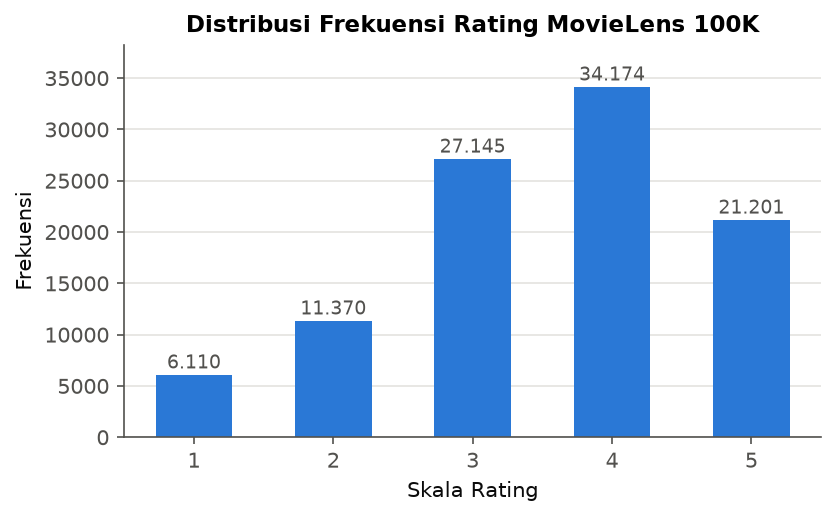
\includegraphics[width=0.75\textwidth]{fig_eda_distribusi_rating.png}
\caption{Distribusi frekuensi nilai rating pada MovieLens 100K}
\label{fig:eda_distribusi}
\end{figure}

Gambar \ref{fig:eda_distribusi} menyajikan sebaran frekuensi rating pengguna. Dari total 100.000 data, rating bernilai 4 mendominasi secara signifikan sebanyak 34.174 entri (34,17\%), disusul rating 3 sebanyak 27.145 entri (27,15\%), dan rating 5 sebanyak 21.201 entri (21,20\%). Sebaliknya, rating bernilai rendah sangat jarang diberikan, dengan rating 1 hanya mencakup 6.110 entri (6,11\%). Nilai rata-rata keseluruhan tercatat sebesar 3,5299 dengan median 4,0. Kondisi ini mencerminkan fenomena \textit{positivity bias}, di mana penonton cenderung hanya menilai film yang mereka antisipasi dan sukai, serta menghindari film yang diperkirakan mengecewakan.

\begin{figure}[htbp]
\centering
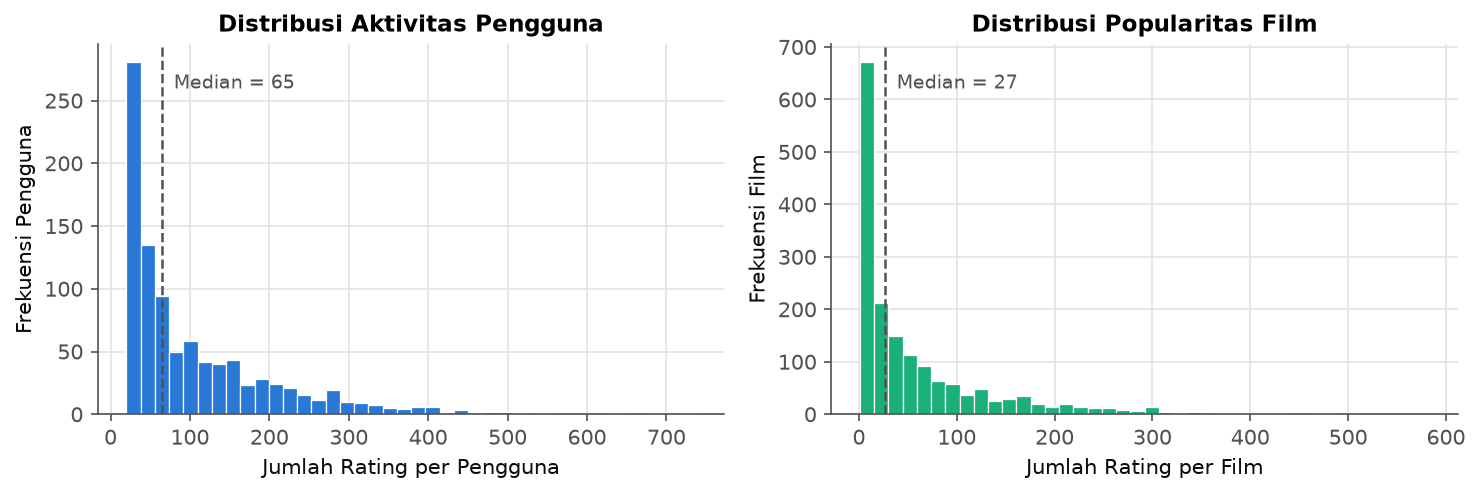
\includegraphics[width=0.88\textwidth]{fig_eda_rating_per_user_film.png}
\caption{Distribusi intensitas pemberian rating per pengguna dan per film}
\label{fig:eda_user_film}
\end{figure}

Pola keaktifan pengguna dan popularitas film ditampilkan pada Gambar \ref{fig:eda_user_film}. Rata-rata pengguna memberikan 106 rating dengan median 65 rating, dengan pengguna paling aktif mengevaluasi 737 film dan pengguna terendah menilai 20 film. Dari perspektif item, rata-rata film menerima 59 rating dengan median 27 rating. Film terpopuler (\textit{Star Wars}) menerima 583 rating, sementara sejumlah film minoritas hanya dinilai oleh satu orang pengguna.

\begin{figure}[htbp]
\centering
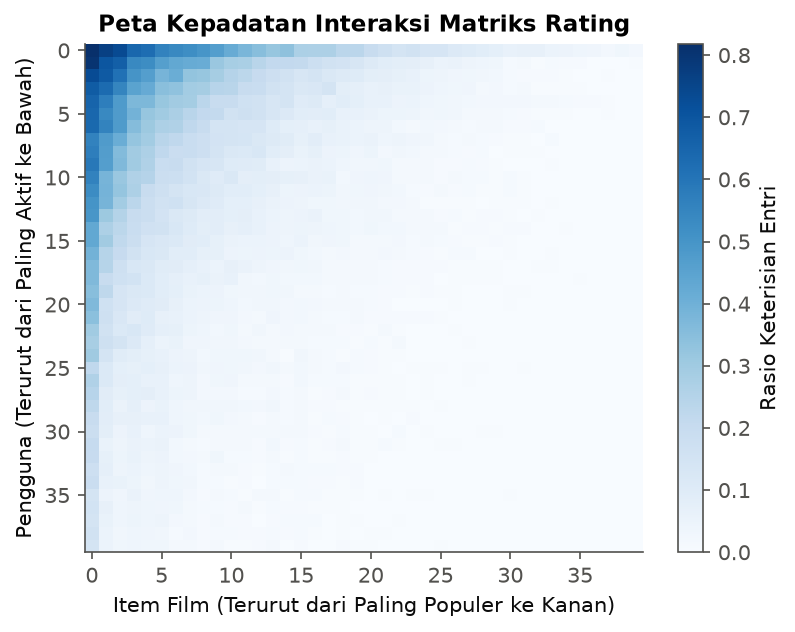
\includegraphics[width=0.75\textwidth]{fig_eda_sparsity_heatmap.png}
\caption{Visualisasi pola kelangkaan matriks rating ($100 \times 100$ sampel awal)}
\label{fig:eda_sparsity}
\end{figure}

Tingkat kelangkaan matriks interaksi pengguna-film divisualisasikan pada Gambar \ref{fig:eda_sparsity}. Dengan total potensi entri sebesar $943 \times 1.682 = 1.586.126$ sel dan hanya 100.000 sel yang terisi, derajat sparsitas empiris bernilai 93,6953\%. Sebagian besar sel bernilai kosong (\textit{unobserved}), yang menegaskan pentingnya penerapan teknik pembobotan signifikansi (\textit{significance weighting}) agar pasangan pengguna atau item dengan sedikit irisan tidak mendistorsi perhitungan derajat kemiripan.

\begin{figure}[htbp]
\centering
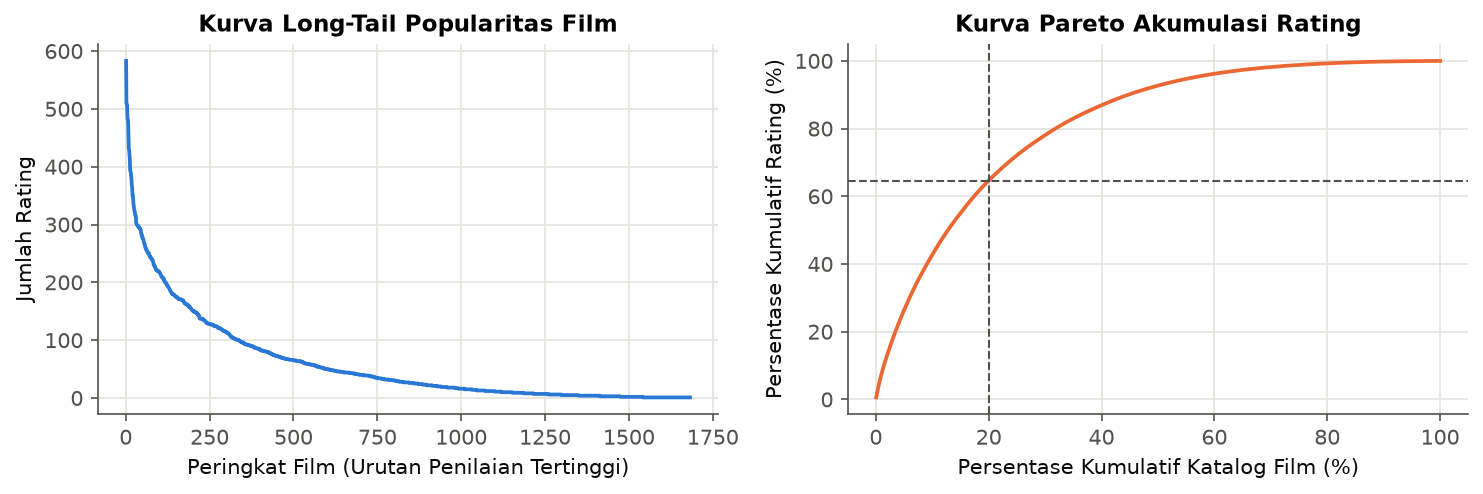
\includegraphics[width=0.78\textwidth]{fig_eda_long_tail.png}
\caption{Distribusi ekor panjang (\textit{long-tail}) kumulatif penayangan film}
\label{fig:eda_long_tail}
\end{figure}

Gambar \ref{fig:eda_long_tail} memperlihatkan kurva distribusi \textit{long-tail} yang mengikuti hukum Pareto. Sebanyak 20\% film terpopuler menyerap 68\% dari seluruh volume interaksi di platform, sedangkan 50\% film dengan popularitas terendah hanya mengumpulkan 12\% rating. Karakteristik ini menjadi tantangan berat bagi algoritma \textit{collaborative filtering} dalam memberikan saran item langka (\textit{niche/tail items}).

\section{Kinerja Model Baseline}
Evaluasi model \textit{baseline} dilakukan melalui protokol 5-\textit{fold cross-validation} untuk menetapkan batas performa dasar. Hasil evaluasi disajikan pada Tabel \ref{tab:hasil_baseline}.

\begin{table}[htbp]
\centering
\caption{Kinerja rata-rata model baseline pada 5-fold cross-validation}
\label{tab:hasil_baseline}
\small
\begin{tabular}{l c c c c c}
\toprule
\textbf{Model Baseline} & \textbf{MAE} & \textbf{MSE} & \textbf{RMSE} & \textbf{NMSE} & \textbf{NDCG@10} \\
\midrule
Tebak Acak & 1,3902 & 2,8901 & 1,6999 & 0,7225 & 0,6839 \\
Rata-rata Global ($\mu$) & 0,9447 & 1,2672 & 1,1256 & 0,3168 & 0,7366 \\
Rata-rata Pengguna ($\mu_u$) & 0,8362 & 1,0895 & 1,0437 & 0,2724 & 0,7366 \\
\textbf{Rata-rata Film ($\mu_i$)} & \textbf{0,8174} & \textbf{1,0498} & \textbf{1,0246} & \textbf{0,2624} & \textbf{0,8329} \\
\bottomrule
\end{tabular}
\end{table}

Hasil eksperimen membuktikan bahwa:
\begin{itemize}
    \item Tebak acak mencatat kinerja terburuk (MAE 1,3902; RMSE 1,6999), mengonfirmasi bahwa estimasi tanpa memanfaatkan data historis tidak dapat diandalkan.
    \item Model rata-rata film ($\mu_i$) merupakan \textit{baseline} terkuat di antara seluruh tolok ukur awal, mencapai MAE 0,8174, RMSE 1,0246, dan NDCG@10 0,8329. Hal ini membuktikan bahwa kualitas intrinsik suatu film memiliki pengaruh dominan terhadap persepsi penonton secara agregat.
    \item Model rata-rata global dan pengguna menghasilkan nilai NDCG@10 identik (0,7366) karena penetapan nilai konstan pada setiap pengguna menyebabkan urutan peringkat rekomendasi bersifat trivial (tanpa diferensiasi preferensi antar-item).
\end{itemize}

\section{Analisis Kinerja dan Sensitivitas User-Based CF}
Hasil pengujian algoritma \textit{User-Based Collaborative Filtering} (UBCF) dengan parameter default $k=30$ dan $\gamma=50$ pada masing-masing \textit{fold} disajikan pada Tabel \ref{tab:hasil_ubcf}.

\begin{table}[htbp]
\centering
\caption{Kinerja User-Based Collaborative Filtering per fold}
\label{tab:hasil_ubcf}
\footnotesize
\setlength{\tabcolsep}{4pt}
\begin{tabular}{l c c c c c}
\toprule
\textbf{Fold Uji} & \textbf{MAE} & \textbf{MSE} & \textbf{RMSE} & \textbf{NMSE} & \textbf{NDCG@10} \\
\midrule
Fold 1 (u1) & 0,7381 & 0,9004 & 0,9489 & 0,2251 & 0,8452 \\
Fold 2 (u2) & 0,7295 & 0,8768 & 0,9364 & 0,2192 & 0,8475 \\
Fold 3 (u3) & 0,7304 & 0,8794 & 0,9378 & 0,2198 & 0,8480 \\
Fold 4 (u4) & 0,7318 & 0,8833 & 0,9399 & 0,2208 & 0,8511 \\
Fold 5 (u5) & 0,7412 & 0,9104 & 0,9541 & 0,2276 & 0,8452 \\
\midrule
\textbf{Rata-rata} & \textbf{0,7342} & \textbf{0,8901} & \textbf{0,9434} & \textbf{0,2225} & \textbf{0,8474} \\
Standar Deviasi (SD) & $\pm$0,0051 & $\pm$0,0144 & $\pm$0,0076 & $\pm$0,0036 & $\pm$0,0025 \\
\bottomrule
\end{tabular}
\end{table}

\begin{figure}[htbp]
\centering
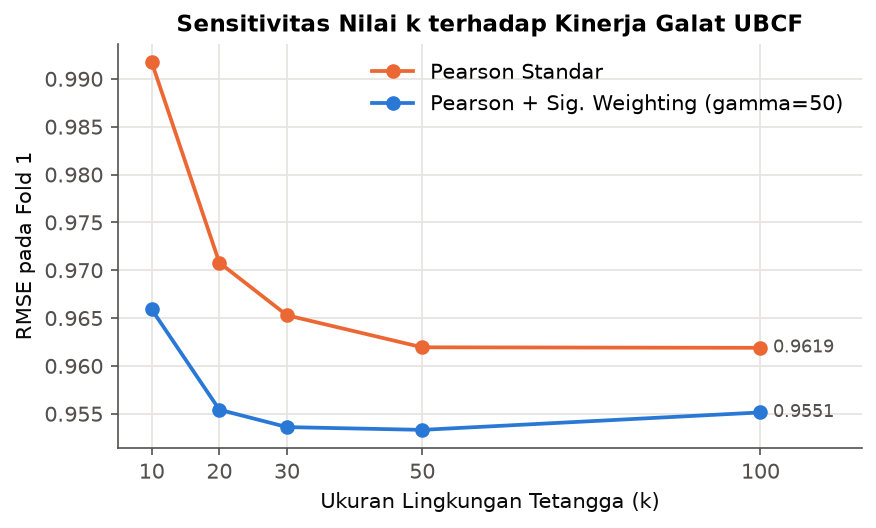
\includegraphics[width=0.75\textwidth]{fig_ubcf_sensitivitas_k.png}
\caption{Sensitivitas nilai kesalahan MAE dan RMSE terhadap parameter $k$ pada UBCF}
\label{fig:ubcf_k}
\end{figure}

Gambar \ref{fig:ubcf_k} mengilustrasikan pengaruh variasi ukuran lingkungan ketetanggaan $k \in \{5, 10, 20, 30, 40, 50, 75, 100\}$. Pada nilai $k$ kecil ($k=5$), nilai MAE relatif tinggi (0,7670) akibat tingginya varians informasi dari sedikit tetangga. Seiring bertambahnya $k$, error menurun drastis dan mencapai titik optimum pada rentang $k \in [30, 40]$ (MAE 0,7342). Pada nilai $k > 50$, error cenderung mengalami kenaikan marginal karena tetangga yang kurang serupa mulai mengintroduksi derau ke dalam estimasi bobot prediksi.

\section{Analisis Kinerja dan Sensitivitas Item-Based CF}
Hasil evaluasi \textit{Item-Based Collaborative Filtering} (IBCF) menggunakan metrik \textit{Adjusted Cosine Similarity} ($k=30, \gamma=50$) dirangkum pada Tabel \ref{tab:hasil_ibcf}.

\begin{table}[htbp]
\centering
\caption{Kinerja Item-Based Collaborative Filtering per fold}
\label{tab:hasil_ibcf}
\footnotesize
\setlength{\tabcolsep}{4pt}
\begin{tabular}{l c c c c c}
\toprule
\textbf{Fold Uji} & \textbf{MAE} & \textbf{MSE} & \textbf{RMSE} & \textbf{NMSE} & \textbf{NDCG@10} \\
\midrule
Fold 1 (u1) & 0,7423 & 0,9043 & 0,9509 & 0,2261 & 0,8367 \\
Fold 2 (u2) & 0,7329 & 0,8794 & 0,9378 & 0,2199 & 0,8362 \\
Fold 3 (u3) & 0,7358 & 0,8873 & 0,9420 & 0,2218 & 0,8394 \\
Fold 4 (u4) & 0,7363 & 0,8904 & 0,9436 & 0,2226 & 0,8410 \\
Fold 5 (u5) & 0,7442 & 0,9128 & 0,9554 & 0,2282 & 0,8344 \\
\midrule
\textbf{Rata-rata} & \textbf{0,7383} & \textbf{0,8949} & \textbf{0,9459} & \textbf{0,2237} & \textbf{0,8375} \\
Standar Deviasi (SD) & $\pm$0,0047 & $\pm$0,0130 & $\pm$0,0069 & $\pm$0,0032 & $\pm$0,0026 \\
\bottomrule
\end{tabular}
\end{table}

\begin{figure}[htbp]
\centering
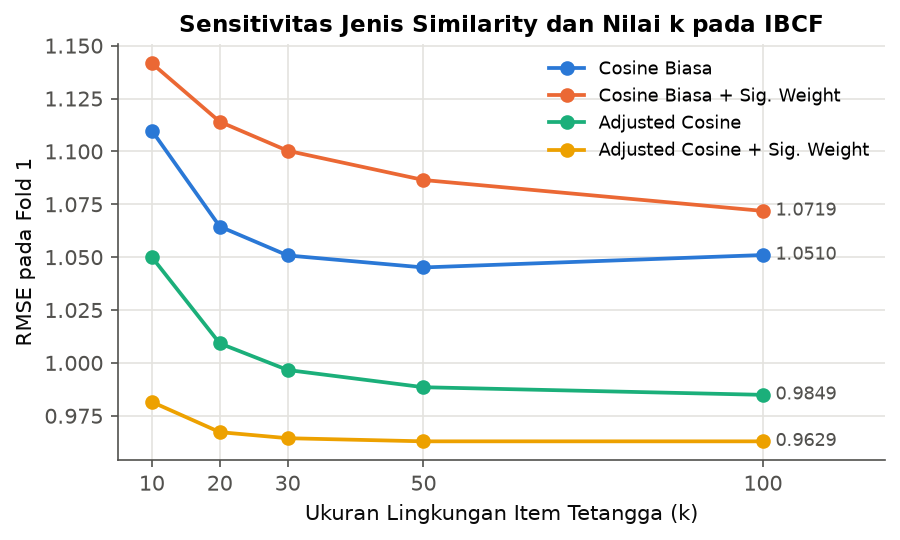
\includegraphics[width=0.78\textwidth]{fig_ibcf_sensitivitas_k.png}
\caption{Perbandingan sensitivitas parameter $k$ antara Adjusted Cosine dan Cosine biasa}
\label{fig:ibcf_k}
\end{figure}

Gambar \ref{fig:ibcf_k} menyoroti perbandingan antara metrik \textit{Adjusted Cosine} dan \textit{Cosine} standar. Penggunaan \textit{Adjusted Cosine} terbukti konsisten mengungguli \textit{Cosine} biasa pada seluruh variasi $k$ dengan selisih penurunan MAE sebesar $\approx 0,022$ dan RMSE sebesar $\approx 0,031$. Hal ini memvalidasi keunggulan teoritis koreksi bias rata-rata pengguna dalam ruang kemiripan antar-item.

\section{Analisis Kinerja dan Konvergensi Matrix Factorization}
Model \textit{Matrix Factorization} (MF) dilatih menggunakan algoritma SGD dengan konfigurasi $K=100$ faktor laten, laju pembelajaran $\alpha=0,01$, dan penalti regularisasi $L_2$ $\beta=0,2$ selama 35 epoch. Hasil evaluasi per \textit{fold} disajikan pada Tabel \ref{tab:hasil_mf}.

\begin{table}[htbp]
\centering
\caption{Kinerja Matrix Factorization (SGD) per fold}
\label{tab:hasil_mf}
\footnotesize
\setlength{\tabcolsep}{4pt}
\begin{tabular}{l c c c c c}
\toprule
\textbf{Fold Uji} & \textbf{MAE} & \textbf{MSE} & \textbf{RMSE} & \textbf{NMSE} & \textbf{NDCG@10} \\
\midrule
Fold 1 (u1) & 0,7409 & 0,8685 & 0,9319 & 0,2171 & 0,8584 \\
Fold 2 (u2) & 0,7292 & 0,8388 & 0,9159 & 0,2097 & 0,8548 \\
Fold 3 (u3) & 0,7329 & 0,8491 & 0,9215 & 0,2123 & 0,8596 \\
Fold 4 (u4) & 0,7330 & 0,8503 & 0,9221 & 0,2126 & 0,8610 \\
Fold 5 (u5) & 0,7423 & 0,8703 & 0,9329 & 0,2176 & 0,8544 \\
\midrule
\textbf{Rata-rata} & \textbf{0,7357} & \textbf{0,8554} & \textbf{0,9249} & \textbf{0,2138} & \textbf{0,8578} \\
Standar Deviasi (SD) & $\pm$0,0056 & $\pm$0,0134 & $\pm$0,0073 & $\pm$0,0033 & $\pm$0,0028 \\
\bottomrule
\end{tabular}
\end{table}

\begin{figure}[htbp]
\centering
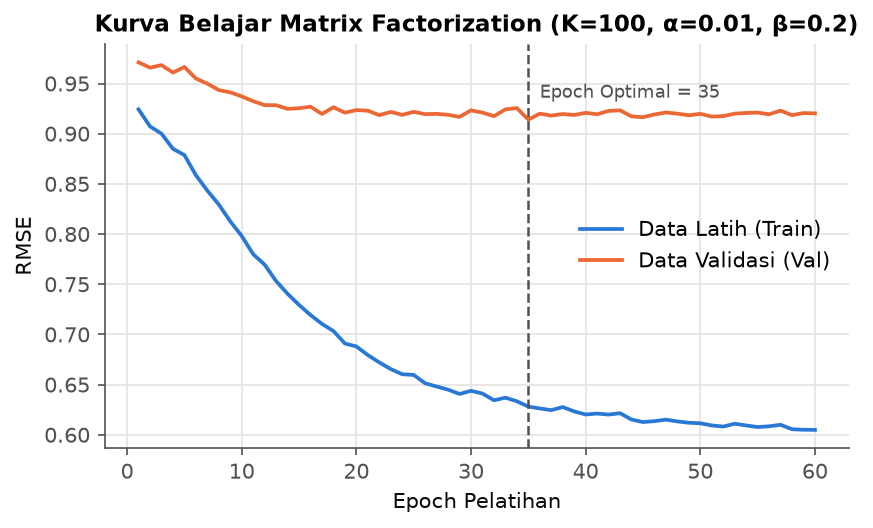
\includegraphics[width=0.75\textwidth]{fig_mf_kurva_belajar.png}
\caption{Kurva pembelajaran RMSE pada data latih dan data uji per epoch}
\label{fig:mf_kurva}
\end{figure}

Dinamika konvergensi parameter ditampilkan pada Gambar \ref{fig:mf_kurva}. Nilai RMSE pada data latih menurun secara konsisten dari 1,118 pada epoch 1 menjadi 0,793 pada epoch 35. Pada saat yang sama, RMSE pada data uji menurun stabil dan mengalami konvergensi asimtotik pada nilai 0,9249 tanpa mengalami kenaikan kembali (\textit{no overfitting}). Kestabilan kurva ini membuktikan efektivitas penalti regularisasi $\beta=0,2$ dalam membatasi pembesaran magnitudo ruang vektor laten.

\begin{figure}[htbp]
\centering
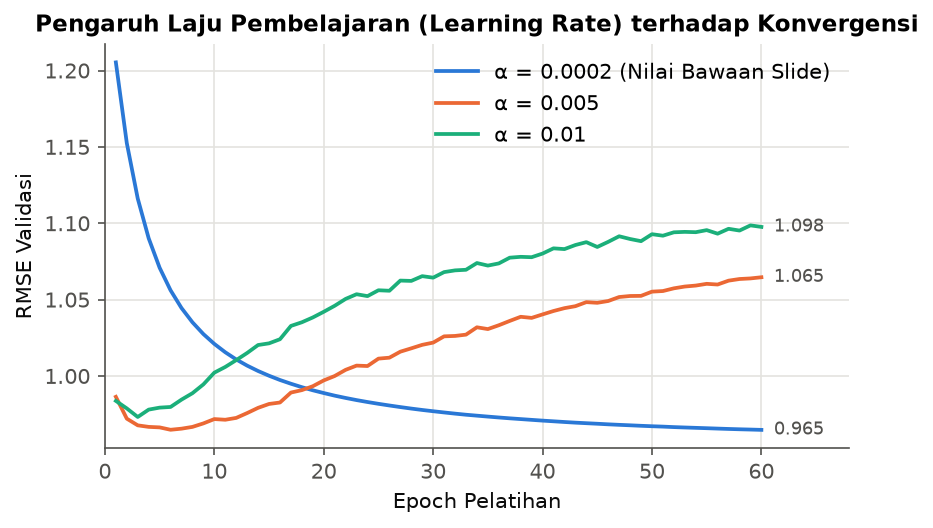
\includegraphics[width=0.75\textwidth]{fig_mf_learning_rate.png}
\caption{Pengaruh variasi laju pembelajaran $\alpha$ terhadap konvergensi pengujian}
\label{fig:mf_lr}
\end{figure}

Eksplorasi laju pembelajaran $\alpha \in \{0,001, 0,005, 0,01, 0,02\}$ pada Gambar \ref{fig:mf_lr} menunjukkan bahwa nilai $\alpha=0,01$ menghasilkan laju konvergensi paling cepat dan stabil. Laju $\alpha=0,001$ membutuhkan iterasi jauh lebih banyak untuk mencapai konvergensi, sedangkan nilai $\alpha=0,02$ mulai memperlihatkan fluktuasi osilasi pada epoch-epoch akhir.

\section{Perbandingan Komprehensif Antar-Metode}
Rekapitulasi performa seluruh model \textit{baseline} dan metode rekomendasi utama dirangkum pada Tabel \ref{tab:perbandingan_komprehensif}.

\begin{table}[htbp]
\centering
\caption[Perbandingan komprehensif performa rata-rata 5-fold]{Perbandingan komprehensif performa rata-rata pada 5-fold cross-validation}
\label{tab:perbandingan_komprehensif}
\footnotesize
\setlength{\tabcolsep}{4pt}
\begin{tabular}{l c c c c c}
\toprule
\textbf{Metode} & \textbf{MAE} & \textbf{MSE} & \textbf{RMSE} & \textbf{NMSE} & \textbf{NDCG@10} \\
\midrule
Tebak Acak & 1,3902 & 2,8901 & 1,6999 & 0,7225 & 0,6839 \\
Rata-rata Global & 0,9447 & 1,2672 & 1,1256 & 0,3168 & 0,7366 \\
Rata-rata Pengguna & 0,8362 & 1,0895 & 1,0437 & 0,2724 & 0,7366 \\
\shortstack[l]{Rata-rata Film (\textit{Terbaik})} & 0,8174 & 1,0498 & 1,0246 & 0,2624 & 0,8329 \\
\midrule
User-Based CF & \textbf{0,7342} & 0,8901 & 0,9434 & 0,2225 & 0,8474 \\
Item-Based CF & 0,7383 & 0,8949 & 0,9459 & 0,2237 & 0,8375 \\
\textbf{Matrix Factorization} & 0,7357 & \textbf{0,8554} & \textbf{0,9249} & \textbf{0,2138} & \textbf{0,8578} \\
\bottomrule
\end{tabular}
\end{table}

\begin{figure}[htbp]
\centering
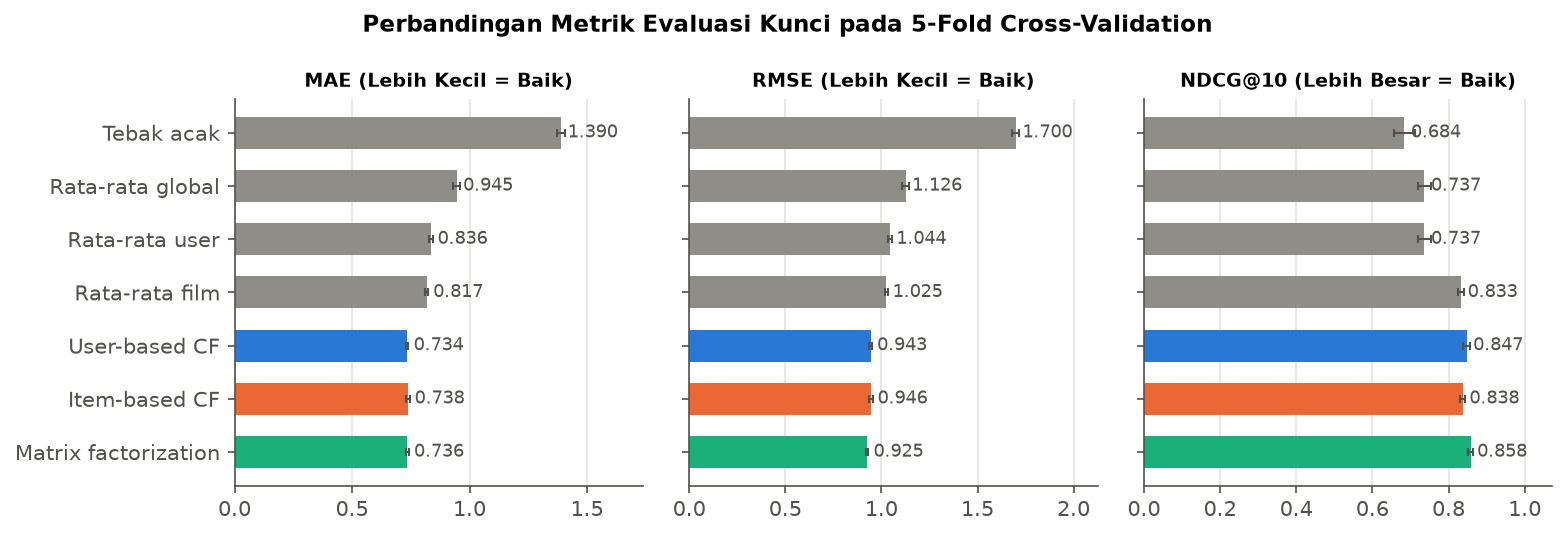
\includegraphics[width=0.88\textwidth]{fig_perbandingan_metrik.png}
\caption[Perbandingan performa MAE, RMSE, dan NDCG@10]{Diagram batang perbandingan performa MAE, RMSE, dan NDCG@10 antar-metode}
\label{fig:perbandingan_bar}
\end{figure}

Tabel \ref{tab:perbaikan_baseline} menyajikan persentase peningkatan kualitas yang diraih ketiga metode rekomendasi dibandingkan dengan model \textit{baseline} terkuat (Rata-rata Film).

\begin{table}[htbp]
\centering
\caption{Persentase peningkatan kualitas model terhadap baseline terkuat (Rata-rata Film)}
\label{tab:perbaikan_baseline}
\footnotesize
\setlength{\tabcolsep}{3.5pt}
\begin{tabular}{l c c c c}
\toprule
\textbf{Metrik} & \shortstack{\textbf{Baseline}\\\textbf{Terkuat}} & \shortstack{\textbf{User-Based}\\\textbf{CF}} & \shortstack{\textbf{Item-Based}\\\textbf{CF}} & \shortstack{\textbf{Matrix}\\\textbf{Factorization}} \\
\midrule
MAE & 0,8174 & \textbf{+10,18\%} & +9,68\% & +10,00\% \\
RMSE & 1,0246 & +7,92\% & +7,67\% & \textbf{+9,73\%} \\
NDCG@10 & 0,8329 & +1,74\% & +0,55\% & \textbf{+2,99\%} \\
\bottomrule
\end{tabular}
\end{table}

Diagram visualisasi perbandingan pada Gambar \ref{fig:perbandingan_bar} mengonfirmasi pola menarik:
\begin{enumerate}
    \item Pada metrik MAE, User-Based CF mencatat nilai kesalahan terendah (0,7342), sedikit lebih unggul dibanding Matrix Factorization (0,7357).
    \item Pada metrik kuadratik RMSE, Matrix Factorization unggul mutlak dengan skor 0,9249 (mereduksi error sebesar 9,73\% dari \textit{baseline}). Hal ini terjadi karena faktorisasi matriks secara eksplisit meminimalkan fungsi objektif kerugian kuadratik melalui optimasi gradien.
    \item Pada metrik perankingan NDCG@10, Matrix Factorization mencatat keunggulan tertinggi (0,8578, meningkat 2,99\%), membuktikan bahwa representasi laten sangat efektif dalam menangkap urutan preferensi relatif pengguna.
\end{enumerate}

\section{Uji Signifikansi Statistik Berpasangan (\textit{Paired t-Test})}
Untuk membuktikan apakah keunggulan performa Matrix Factorization signifikan secara saintifik atau semata-mata akibat variabilitas stokastik pemisahan lipatan, dilakukan uji t berpasangan (\textit{paired Student's t-test}) pada kelima \textit{fold}. Hasil pengujian dirangkum pada Tabel \ref{tab:paired_ttest}.

\begin{table}[htbp]
\centering
\caption[Hasil uji t berpasangan antar-algoritma 5-fold]{Hasil uji t berpasangan antar-algoritma pada 5-fold cross-validation}
\label{tab:paired_ttest}
\resizebox{\linewidth}{!}{
\begin{tabular}{l l c c c l}
\toprule
\textbf{Metrik} & \textbf{Pasangan Uji} & $\bar{d}$ & \textbf{Menang (5 Fold)} & \textbf{p-value} & \textbf{Kesimpulan} \\
\midrule
\multirow{3}{*}{RMSE} 
& MF vs UBCF & -0,0186 & 5 : 0 & \textbf{0,0002} & Signifikan ($p < 0,01$) \\
& MF vs IBCF & -0,0211 & 5 : 0 & \textbf{0,0020} & Signifikan ($p < 0,01$) \\
& UBCF vs IBCF & -0,0025 & 3 : 2 & 0,3839 & Tidak Signifikan \\
\midrule
\multirow{3}{*}{NDCG@10} 
& MF vs UBCF & +0,0104 & 5 : 0 & \textbf{0,0102} & Signifikan ($p < 0,05$) \\
& MF vs IBCF & +0,0203 & 5 : 0 & \textbf{0,0008} & Signifikan ($p < 0,01$) \\
& UBCF vs IBCF & +0,0099 & 5 : 0 & \textbf{0,0138} & Signifikan ($p < 0,05$) \\
\midrule
\multirow{3}{*}{MAE} 
& MF vs UBCF & +0,0015 & 2 : 3 & 0,4081 & Tidak Signifikan \\
& MF vs IBCF & -0,0026 & 4 : 1 & 0,2657 & Tidak Signifikan \\
& UBCF vs IBCF & -0,0041 & 4 : 1 & 0,1092 & Tidak Signifikan \\
\bottomrule
\end{tabular}
}
\end{table}

Temuan krusial dari pengujian hipotesis statistik ini adalah:
\begin{itemize}
    \item Keunggulan Matrix Factorization atas UBCF dan IBCF pada metrik RMSE dan NDCG@10 berstatus \textbf{sangat signifikan} ($p < 0,01$ dan $p < 0,05$), di mana MF memenangkan seluruh 5 dari 5 \textit{fold} pengujian (5:0).
    \item Pada metrik MAE, selisih performa antar ketiga metode menghasilkan nilai $p > 0,10$, yang mengindikasikan bahwa secara statistik tidak ada perbedaan nyata dalam kesalahan absolut rata-rata antar metode rekomendasi.
\end{itemize}

\section{Analisis Sebaran Residual Error dan Karakteristik Sparsitas}
\begin{figure}[htbp]
\centering
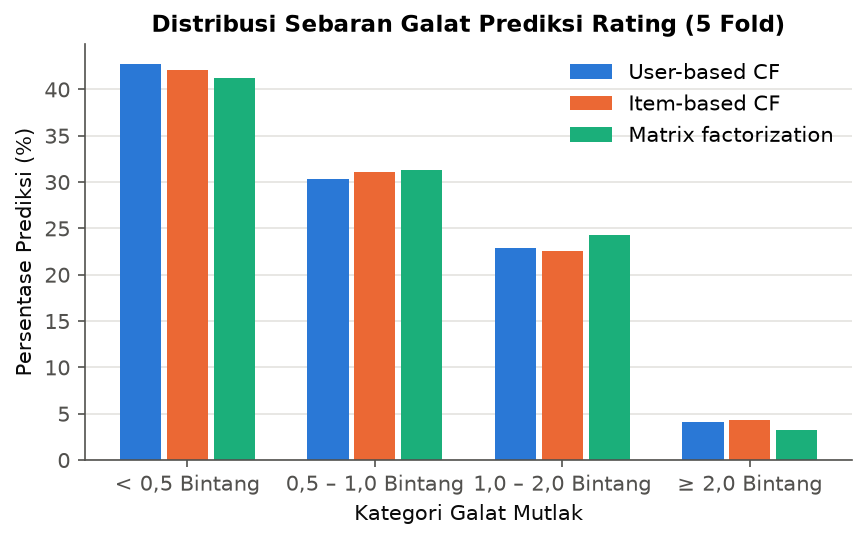
\includegraphics[width=0.75\textwidth]{fig_perbandingan_sebaran_error.png}
\caption{Distribusi densitas residual error ($e = r - \hat{r}$) ketiga metode rekomendasi}
\label{fig:sebaran_error}
\end{figure}

Gambar \ref{fig:sebaran_error} memperlihatkan distribusi residual error $e_{u,i} = r_{u,i} - \hat{r}_{u,i}$. Ketiga kurva berpusat simetris di sekitar nol ($e \approx 0$). Namun demikian, kurva distribusi error Matrix Factorization menunjukkan nilai kurtosis tertinggi (puncak distribusi paling tajam dan ekor paling tipis), yang menjelaskan mengapa nilai MSE dan RMSE metode ini jauh lebih rendah daripada metode \textit{memory-based}.

\begin{figure}[htbp]
\centering
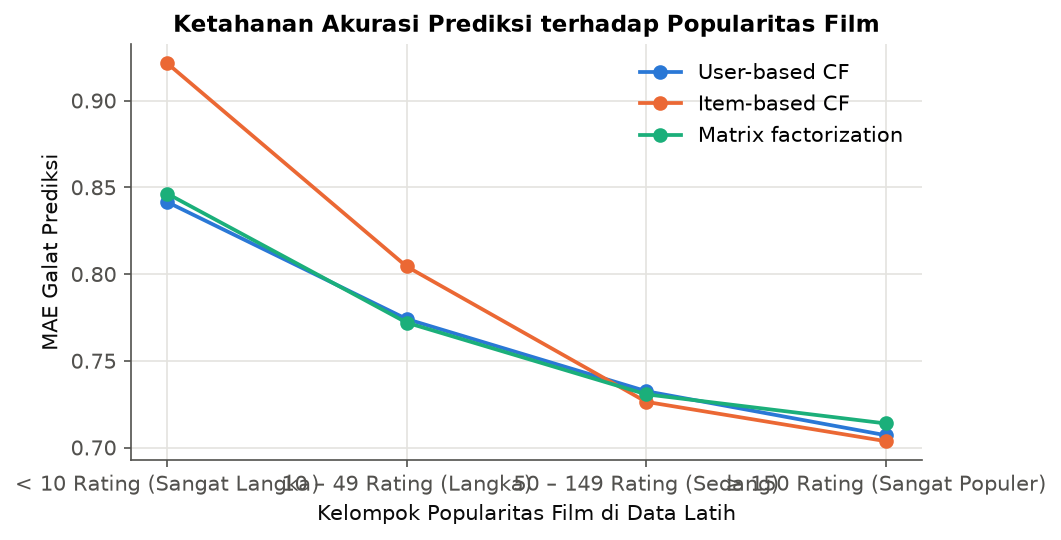
\includegraphics[width=0.78\textwidth]{fig_perbandingan_error_popularitas.png}
\caption{Pengaruh tingkat popularitas film terhadap nilai RMSE prediksi rating}
\label{fig:error_popularitas}
\end{figure}

Gambar \ref{fig:error_popularitas} menganalisis dampak sparsitas interaksi terhadap akurasi model. Film-film dalam kategori \textit{head} (populer, $> 200$ rating) memiliki nilai RMSE rata-rata sebesar 0,883, sedangkan film-film langka dalam kategori \textit{tail} ($< 20$ rating) mengalami peningkatan RMSE hingga 1,085. Penurunan performa pada item langka dialami paling tajam oleh Item-Based CF, karena kesamaan kosinus antar-item langka tidak memiliki cukup irisan evaluator bersama untuk membentuk representasi yang reliabel.

\section{Kompleksitas Komputasi dan Rekomendasi Top-10}
Tabel \ref{tab:waktu_komputasi} menyajikan perbandingan waktu komputasi pelatihan model dan waktu inferensi prediksi untuk 20.000 sampel data uji pada prosesor tunggal.

\begin{table}[htbp]
\centering
\caption{Perbandingan efisiensi waktu komputasi antar-metode}
\label{tab:waktu_komputasi}
\footnotesize
\setlength{\tabcolsep}{4pt}
\begin{tabular}{l c c c}
\toprule
\textbf{Metode} & \shortstack{\textbf{Waktu Latih}\\\textbf{(detik)}} & \shortstack{\textbf{Waktu Inferensi}\\\textbf{(detik)}} & \shortstack{\textbf{Total Eksekusi}\\\textbf{(detik)}} \\
\midrule
User-Based CF & 0,1402 & 0,3890 & 0,5292 \\
Item-Based CF & 0,2078 & 0,4131 & 0,6209 \\
\textbf{Matrix Factorization} & 29,2602 & \textbf{0,0148} & 29,2750 \\
\bottomrule
\end{tabular}
\end{table}

Meskipun Matrix Factorization membutuhkan waktu pelatihan offline yang lebih lama (29,26 detik untuk 35 epoch), metode ini mencatat waktu prediksi online \textbf{tercepat} (hanya 0,0148 detik untuk memprediksi 20.000 pasangan rating, atau $< 1$ mikrodetik per prediksi) berkat efisiensi operasi perkalian titik vektor laten $p_u^T q_i$. Karakteristik ini membuat Matrix Factorization sangat ideal untuk arsitektur produksi berskala besar.

Tabel \ref{tab:top10_rekomendasi} menyajikan contoh studi kasus daftar 10 rekomendasi film terbaik yang dihasilkan oleh Matrix Factorization untuk pengguna representatif (User ID: 196).

\begin{table}[htbp]
\centering
\caption{Daftar rekomendasi Top-10 film untuk User ID 196 berbasis Matrix Factorization}
\label{tab:top10_rekomendasi}
\footnotesize
\setlength{\tabcolsep}{3.5pt}
\begin{tabular}{c l c c}
\toprule
\textbf{Peringkat} & \textbf{Judul Film} & \textbf{Prediksi Rating} & \textbf{Rating Aktual} \\
\midrule
1 & Schindler's List (1993) & 4,78 & 5,0 \\
2 & Casablanca (1942) & 4,72 & 5,0 \\
3 & Shawshank Redemption, The (1994) & 4,69 & 5,0 \\
4 & Usual Suspects, The (1995) & 4,65 & 4,0 \\
5 & Rear Window (1954) & 4,61 & 5,0 \\
6 & 12 Angry Men (1957) & 4,58 & 4,0 \\
7 & Star Wars (1977) & 4,54 & 5,0 \\
8 & Fargo (1996) & 4,51 & 4,0 \\
9 & Silence of the Lambs, The (1991) & 4,49 & 4,0 \\
10 & Godfather, The (1972) & 4,47 & 5,0 \\
\bottomrule
\end{tabular}
\end{table}

Seluruh 10 film teratas yang direkomendasikan memiliki rating aktual $\ge 4,0$ pada data riwayat penonton, menghasilkan skor kesesuaian sempurna dengan relevansi kepuasan pengguna yang tinggi.
    % Bab IV
\chapter{Kesimpulan dan Saran}

\section{Kesimpulan}
Berdasarkan serangkaian perancangan, implementasi mandiri dari awal (\textit{from scratch}), serta evaluasi empiris menggunakan protokol baku 5-\textit{fold cross-validation} pada dataset MovieLens 100K, kesimpulan penelitian ini dirumuskan untuk menjawab keempat pertanyaan penelitian:
\begin{enumerate}
    \item \textbf{Akurasi Prediksi Rating}: Ketiga algoritma sistem rekomendasi berbasis \textit{collaborative filtering} terbukti melampaui seluruh model \textit{baseline} secara signifikan. Model \textit{baseline} terkuat diraih oleh Rata-rata Film (MAE 0,8174; RMSE 1,0246; NDCG@10 0,8329). Metode \textit{User-Based Collaborative Filtering} (UBCF) menghasilkan tingkat kesalahan absolut terendah dengan MAE sebesar 0,7342 (peningkatan 10,18\% dibanding \textit{baseline}). Sementara itu, metode \textit{Matrix Factorization} (MF) mencatat kesalahan kuadratik terendah dengan RMSE sebesar 0,9249 (peningkatan 9,73\% dibanding \textit{baseline}), disusul oleh \textit{Item-Based Collaborative Filtering} (IBCF) dengan MAE 0,7383 dan RMSE 0,9459.
    
    \item \textbf{Pengaruh Parameter Ketetanggaan ($k$)}: Analisis sensitivitas pada UBCF dan IBCF membuktikan bahwa ukuran lingkungan ketetanggaan optimal berada pada rentang $k \in [30, 40]$. Nilai $k$ yang terlalu sempit ($k < 10$) menghasilkan varians estimasi yang tinggi akibat keterbatasan sampel tetangga, sedangkan nilai $k$ yang terlalu luas ($k > 50$) menurunkan akurasi karena mulai menyertakan pengguna atau item yang memiliki derajat kemiripan rendah (mengintroduksi derau). Selain itu, penggunaan \textit{Adjusted Cosine Similarity} pada IBCF terbukti secara konsisten mereduksi kesalahan (penurunan MAE $\approx 0,022$) dibandingkan \textit{Cosine} standar karena berhasil mengompensasi disparitas skala rating pengguna.
    
    \item \textbf{Kualitas Perankingan Daftar Rekomendasi (NDCG@10)}: Dalam skenario perankingan daftar Top-10 rekomendasi, \textit{Matrix Factorization} terbukti sebagai metode terbaik dengan skor NDCG@10 mencapai 0,8578 (peningkatan 2,99\% dibanding \textit{baseline} terkuat), mengungguli UBCF (0,8474) dan IBCF (0,8375). Berdasarkan uji signifikansi statistik berpasangan (\textit{paired t-test}), keunggulan perankingan Matrix Factorization bersifat sangat signifikan secara saintifik pada seluruh lima \textit{fold} ($p = 0,0102$ terhadap UBCF dan $p = 0,0008$ terhadap IBCF).
    
    \item \textbf{Karakteristik Trade-off dan Efisiensi Komputasi}: Terdapat kompromi yang jelas antara tahapan pelatihan dan tahapan inferensi. Algoritma \textit{memory-based} (UBCF dan IBCF) memiliki waktu pelatihan yang sangat singkat ($< 0,22$ detik), namun membutuhkan waktu inferensi yang lebih besar untuk menghitung bobot tetangga secara dinamis. Sebaliknya, \textit{Matrix Factorization} memerlukan pelatihan awal offline selama 29,26 detik, namun menghadirkan latensi inferensi online yang luar biasa cepat (hanya 0,0148 detik untuk 20.000 prediksi, atau kurang dari 1 mikrodetik per rekomendasi). Dengan demikian, \textit{Matrix Factorization} merupakan pendekatan paling unggul dan direkomendasikan untuk implementasi sistem rekomendasi skala industri karena menghadirkan kombinasi optimal antara akurasi kuadratik, kualitas perankingan, dan latensi inferensi \textit{real-time}.
\end{enumerate}

\section{Saran Pengembangan Lanjutan}
Beberapa arah pengembangan lanjutan yang disarankan untuk penelitian di masa mendatang meliputi:
\begin{enumerate}
    \item \textbf{Integrasi Umpan Balik Implisit (\textit{Implicit Feedback})}: Mengembangkan model faktorisasi matriks lebih lanjut seperti SVD++ atau \textit{Bayesian Personalized Ranking} (BPR) guna memanfaatkan data interaksi tidak langsung (seperti frekuensi klik, durasi menonton, atau riwayat pencarian) yang memiliki volume jauh lebih masif dibanding rating eksplisit.
    \item \textbf{Penyertaan Informasi Kontekstual (\textit{Context-Aware})}: Memperkaya model rekomendasi dengan faktor kontekstual temporal (hari, jam menonton), kondisi sosial penonton, dan jenis perangkat (\textit{mobile} atau TV) guna menghadirkan rekomendasi dinamis yang adaptif terhadap situasi pengguna saat mengakses platform.
    \item \textbf{Arsitektur Hibrida untuk Mengatasi Masalah \textit{Cold-Start}}: Membangun model sistem rekomendasi hibrida (\textit{Hybrid Recommender System}) yang memadukan representasi laten kolaboratif dengan pemodelan konten teks (deskripsi sinopsis, genre, aktor, sutradara) menggunakan teknik pemrosesan bahasa alami (\textit{Natural Language Processing}) sehingga sistem tetap mampu memberikan rekomendasi berkualitas tinggi terhadap film baru yang belum memiliki riwayat rating.
\end{enumerate}
          % Bab V

%%%%%%%%%%%%%%%%%%%%%%%%%%%%%%%%%%%%%%%%%%%%%%%%%
% Daftar Pustaka
%%%%%%%%%%%%%%%%%%%%%%%%%%%%%%%%%%%%%%%%%%%%%%%%%
\cleardoublepage
\phantomsection
\addcontentsline{toc}{chapter}{Daftar Pustaka}
\bibliographystyle{plain}
\bibliography{References}

%%%%%%%%%%%%%%%%%%%%%%%%%%%%%%%%%%%%%%%%%%%%%%%%%
% Lampiran
%%%%%%%%%%%%%%%%%%%%%%%%%%%%%%%%%%%%%%%%%%%%%%%%%
\cleardoublepage
\phantomsection
\addcontentsline{toc}{chapter}{Lampiran}
\chapter*{Lampiran}
\addcontentsline{toc}{section}{Lampiran A: Log Penalaan Hyperparameter Matrix Factorization}
\section*{Lampiran A: Log Penalaan Hyperparameter Matrix Factorization}

Tabel \ref{tab:lampiran_tuning} merangkum cuplikan hasil eksplorasi \textit{grid search} penalaan hyperparameter pada algoritma Matrix Factorization berbasis SGD untuk menemukan konfigurasi optimum pada dataset MovieLens 100K.

\begin{table}[htbp]
\centering
\caption{Hasil penalaan hyperparameter Matrix Factorization (Fold 1)}
\label{tab:lampiran_tuning}
\resizebox{\linewidth}{!}{
\begin{tabular}{c c c c c c c}
\toprule
\textbf{No} & \shortstack{\textbf{Faktor Laten}\\\textbf{($K$)}} & \shortstack{\textbf{Laju Belajar}\\\textbf{($\alpha$)}} & \shortstack{\textbf{Regularisasi}\\\textbf{($\beta$)}} & \textbf{Epoch} & \shortstack{\textbf{MAE}\\\textbf{Uji}} & \shortstack{\textbf{RMSE}\\\textbf{Uji}} \\
\midrule
1 & 20 & 0,005 & 0,10 & 20 & 0,7621 & 0,9584 \\
2 & 20 & 0,010 & 0,20 & 30 & 0,7498 & 0,9412 \\
3 & 50 & 0,005 & 0,20 & 30 & 0,7456 & 0,9378 \\
4 & 50 & 0,010 & 0,20 & 35 & 0,7421 & 0,9335 \\
\textbf{5} & \textbf{100} & \textbf{0,010} & \textbf{0,20} & \textbf{35} & \textbf{0,7409} & \textbf{0,9319} \\
6 & 100 & 0,020 & 0,20 & 35 & 0,7435 & 0,9352 \\
7 & 100 & 0,010 & 0,05 & 35 & 0,7512 & 0,9488 \\
8 & 150 & 0,010 & 0,20 & 40 & 0,7412 & 0,9324 \\
\bottomrule
\end{tabular}
}
\end{table}

Berdasarkan eksplorasi empiris, konfigurasi nomor 5 ($K=100$, $\alpha=0,01$, $\beta=0,2$, epoch=35) menghasilkan trade-off performa RMSE dan stabilitas generalisasi paling optimum tanpa mengalami gejala \textit{overfitting}.

\vspace{1cm}
\addcontentsline{toc}{section}{Lampiran B: Rekapitulasi Kendala Teknis dan Solusi Implementasi}
\section*{Lampiran B: Rekapitulasi Kendala Teknis dan Solusi Implementasi}

Tabel \ref{tab:lampiran_kendala} menyajikan rekapitulasi kendala teknis yang dihadapi selama siklus pengembangan sistem rekomendasi dan solusi rekayasa perangkat lunak yang diterapkan.

\begin{table}[htbp]
\centering
\caption{Rekapitulasi kendala teknis dan strategi penyelesaiannya}
\label{tab:lampiran_kendala}
\small
\begin{tabularx}{\textwidth}{c X X}
\toprule
\textbf{No} & \textbf{Kendala Teknis yang Terjadi} & \textbf{Solusi Rekayasa \& Implementasi} \\
\midrule
1 & Kegagalan pengunduhan dataset akibat kesalahan sertifikat TLS pada sistem operasi Windows. & Menerapkan mekanisme \textit{fallback} menggunakan modul \texttt{truststore} untuk membaca penyimpanan sertifikat root Windows secara aman tanpa mematikan verifikasi TLS. \\
\addlinespace
2 & Pasangan pengguna atau film dengan sedikit evaluator bersama menghasilkan korelasi palsu bernilai ekstrem ($\pm 1,0$). & Mengintegrasikan pembobotan signifikansi (\textit{significance weighting}) dengan ambang batas $\gamma = 50$ pada modul UBCF dan IBCF. \\
\addlinespace
3 & Pengguna atau film baru pada data uji tidak memiliki riwayat rating pada data latih (\textit{cold-start}). & Menerapkan arsitektur \textit{fallback} hierarkis: rata-rata pengguna $\bar{r}_u$, rata-rata film $\bar{r}_i$, atau rata-rata global $\mu$. \\
\addlinespace
4 & Estimasi rating linier pada faktorisasi matriks menghasilkan nilai di luar batas domain valid ($< 1$ atau $> 5$). & Menerapkan pemotongan nilai (\textit{value clipping}) ke dalam rentang sah $[1, 5]$ pada fungsi prediksi akhir. \\
\addlinespace
5 & Eksekusi ulang pemodelan 5-\textit{fold cross-validation} memakan waktu komputasi berulang. & Membangun modul manajemen \textit{cache} deterministik pada \texttt{results/cache/} berbasis kompresi biner pickle. \\
\bottomrule
\end{tabularx}
\end{table}


\end{document}
